% Options for packages loaded elsewhere
\PassOptionsToPackage{unicode}{hyperref}
\PassOptionsToPackage{hyphens}{url}
\PassOptionsToPackage{dvipsnames,svgnames,x11names}{xcolor}
%
\documentclass[
  12pt,
]{article}
\usepackage{amsmath,amssymb}
\usepackage{iftex}
\ifPDFTeX
  \usepackage[T1]{fontenc}
  \usepackage[utf8]{inputenc}
  \usepackage{textcomp} % provide euro and other symbols
\else % if luatex or xetex
  \usepackage{unicode-math} % this also loads fontspec
  \defaultfontfeatures{Scale=MatchLowercase}
  \defaultfontfeatures[\rmfamily]{Ligatures=TeX,Scale=1}
\fi
\usepackage{lmodern}
\ifPDFTeX\else
  % xetex/luatex font selection
\fi
% Use upquote if available, for straight quotes in verbatim environments
\IfFileExists{upquote.sty}{\usepackage{upquote}}{}
\IfFileExists{microtype.sty}{% use microtype if available
  \usepackage[]{microtype}
  \UseMicrotypeSet[protrusion]{basicmath} % disable protrusion for tt fonts
}{}
\makeatletter
\@ifundefined{KOMAClassName}{% if non-KOMA class
  \IfFileExists{parskip.sty}{%
    \usepackage{parskip}
  }{% else
    \setlength{\parindent}{0pt}
    \setlength{\parskip}{6pt plus 2pt minus 1pt}}
}{% if KOMA class
  \KOMAoptions{parskip=half}}
\makeatother
\usepackage{xcolor}
\usepackage[margin=1in]{geometry}
\usepackage{graphicx}
\makeatletter
\def\maxwidth{\ifdim\Gin@nat@width>\linewidth\linewidth\else\Gin@nat@width\fi}
\def\maxheight{\ifdim\Gin@nat@height>\textheight\textheight\else\Gin@nat@height\fi}
\makeatother
% Scale images if necessary, so that they will not overflow the page
% margins by default, and it is still possible to overwrite the defaults
% using explicit options in \includegraphics[width, height, ...]{}
\setkeys{Gin}{width=\maxwidth,height=\maxheight,keepaspectratio}
% Set default figure placement to htbp
\makeatletter
\def\fps@figure{htbp}
\makeatother
\setlength{\emergencystretch}{3em} % prevent overfull lines
\providecommand{\tightlist}{%
  \setlength{\itemsep}{0pt}\setlength{\parskip}{0pt}}
\setcounter{secnumdepth}{5}
% definitions for citeproc citations
\NewDocumentCommand\citeproctext{}{}
\NewDocumentCommand\citeproc{mm}{%
  \begingroup\def\citeproctext{#2}\cite{#1}\endgroup}
\makeatletter
 % allow citations to break across lines
 \let\@cite@ofmt\@firstofone
 % avoid brackets around text for \cite:
 \def\@biblabel#1{}
 \def\@cite#1#2{{#1\if@tempswa , #2\fi}}
\makeatother
\newlength{\cslhangindent}
\setlength{\cslhangindent}{1.5em}
\newlength{\csllabelwidth}
\setlength{\csllabelwidth}{3em}
\newenvironment{CSLReferences}[2] % #1 hanging-indent, #2 entry-spacing
 {\begin{list}{}{%
  \setlength{\itemindent}{0pt}
  \setlength{\leftmargin}{0pt}
  \setlength{\parsep}{0pt}
  % turn on hanging indent if param 1 is 1
  \ifodd #1
   \setlength{\leftmargin}{\cslhangindent}
   \setlength{\itemindent}{-1\cslhangindent}
  \fi
  % set entry spacing
  \setlength{\itemsep}{#2\baselineskip}}}
 {\end{list}}
\usepackage{calc}
\newcommand{\CSLBlock}[1]{\hfill\break\parbox[t]{\linewidth}{\strut\ignorespaces#1\strut}}
\newcommand{\CSLLeftMargin}[1]{\parbox[t]{\csllabelwidth}{\strut#1\strut}}
\newcommand{\CSLRightInline}[1]{\parbox[t]{\linewidth - \csllabelwidth}{\strut#1\strut}}
\newcommand{\CSLIndent}[1]{\hspace{\cslhangindent}#1}
\ifLuaTeX
\usepackage[bidi=basic]{babel}
\else
\usepackage[bidi=default]{babel}
\fi
\babelprovide[main,import]{spanish}
% get rid of language-specific shorthands (see #6817):
\let\LanguageShortHands\languageshorthands
\def\languageshorthands#1{}
\usepackage{float}
\usepackage{subfig}
\ifLuaTeX
  \usepackage{selnolig}  % disable illegal ligatures
\fi
\usepackage{bookmark}
\IfFileExists{xurl.sty}{\usepackage{xurl}}{} % add URL line breaks if available
\urlstyle{same}
\hypersetup{
  pdftitle={Métodos Para el Cálculo de Reservas de IBNR},
  pdfauthor={Ignacio Campón \& Joaquín Viola},
  pdflang={es},
  colorlinks=true,
  linkcolor={blue},
  filecolor={Maroon},
  citecolor={blue},
  urlcolor={blue},
  pdfcreator={LaTeX via pandoc}}

\title{Métodos Para el Cálculo de Reservas de IBNR}
\usepackage{etoolbox}
\makeatletter
\providecommand{\subtitle}[1]{% add subtitle to \maketitle
  \apptocmd{\@title}{\par {\large #1 \par}}{}{}
}
\makeatother
\subtitle{Seguros Generales y Modelos de Riesgo}
\author{Ignacio Campón \& Joaquín Viola}
\date{}

\begin{document}
\maketitle

\maketitle

\thispagestyle{empty} % Hide header and footer on the title page
\vspace*{\fill} % Pushes content to the bottom of the page
\begin{center}

\includegraphics[width=16cm]{imagenes/logo_inst_80.png}\\[1cm] % Adjust image placement
\end{center}

\newpage

\section{Resúmen}\label{resuxfamen}

En el ámbito de los seguros, las reservas se refiere a la cantidad de
dinero que las compañias aseguradoras deben reservar para poder cumplir
con sus obligaciones de pago a futuro, el cálculo del monto de estas
reservas vienen asociados a una cierta probabilidad de quiebra de la
compañía según el comportamiento aleatorio de los siniestros. En este
trabajo se pretende abordar distintos métodos para el cálculo de
reservas técnicas asociadas al IBNR. El IBNR por sus siglas en inglés,
son los siniestros incurridos y que aún no fueron reclamados. En muchos
países, los seguros de responsabilidad civil cuentan con un período de
10 años para el reclamo de un seguro luego de que el siniestro haya
ocurrido.

En el repositorio
\url{https://github.com/joaquin-viola/Seguros_Generales} se encuentran
los datos utilizados durante el documento, así como el documento en
formato \texttt{RMarkdown} para poder reproducir los códigos utilizados.

\newpage

\tableofcontents

\newpage

\section{Introducción}\label{introducciuxf3n}

Como se comentó en el resúmen, las compañías de seguro a menudo reciben
reclamos por un siniestro durante los años posteriores a la ocurrencia
del mismo, por lo que es necesario contar con las reservas de IBNR, el
fin principal de estas es poder estar cubierto en el futuro de
siniestros que ocurrieron en el año corriente (mientras está activa la
poliza), pero el reclamo es efectuado en los años siguientes.

Para poder calcular las reservas de IBNR hay varios métodos que están
basados en la utilización de información previa (recolectada en años
anteriores), para poder predecir cómo se comportan los reclamos en los
años siguientes.

Se suele trabajar con 3 matrices triangulares, donde las filas son años,
y las columnas son los años transcurridos. Observesé el cuadro
\ref{tabla1}, en la última fila se encuentra el último año, el cuál se
tiene datos para una sola columna, el año corriente. La fila anterior
tendrá una columna más, es decir tendrá información de dos períodos
transcurridos, de esta manera se llega a la primer fila, la cuál es el
último año que se tiene en cuenta, y para el cual se tiene información
de todos los años transcurridos, de esta manera queda explicada la forma
de la matriz triangular.

\begin{table}[ht]
\centering
\caption{Siniestros incurridos acumulados por año y por período transcurrido en pesos.} 
\label{tabla1}
\begingroup\fontsize{8.5pt}{10pt}\selectfont
\begin{tabular}{ccccccccccc}
  \hline
 & 1 & 2 & 3 & 4 & 5 & 6 & 7 & 8 & 9 & 10 \\ 
  \hline
1999 & 652799 & 1383776 & 2634200 & 3167840 & 3842289 & 4029679 & 4454460 & 4817622 & 5012751 & 5099688 \\ 
  2000 & 1360795 & 2480988 & 2806387 & 3592401 & 3451088 & 3931688 & 4491687 & 4165270 & 4221137 &  \\ 
  2001 & 1985553 & 3275646 & 3290023 & 3945474 & 4961886 & 4975029 & 5914580 & 5969088 &  &  \\ 
  2002 & 2901555 & 4528347 & 4556763 & 5790821 & 6444829 & 7957380 & 8581805 &  &  &  \\ 
  2003 & 3572829 & 4717083 & 5937065 & 6835232 & 7309686 & 7276239 &  &  &  &  \\ 
  2004 & 2578343 & 4423917 & 4664371 & 5348014 & 5882585 &  &  &  &  &  \\ 
  2005 & 4051902 & 6081465 & 8618348 & 9901076 &  &  &  &  &  &  \\ 
  2006 & 5030173 & 8881224 & 12548654 &  &  &  &  &  &  &  \\ 
  2007 & 6849422 & 9171465 &  &  &  &  &  &  &  &  \\ 
  2008 & 10120889 &  &  &  &  &  &  &  &  &  \\ 
   \hline
\end{tabular}
\endgroup
\end{table}

La primer matriz triangular tiene la información de los pagos acumulados
de los siniestros ocurridos en cada año, y cuando fueron pagados
efectivamente. Para la primer fila, en la primer columna se tienen los
pagos de los siniestros ocurridos y pagados hace 10 años, luego en la
siguiente columna se tiene los siniestros ocurridos en ese año pero
reclamados y pagados en el siguiente, más los de la columna anterior
(por ser pagos acumulados) y así sucesivamente.

La segunda matriz es la matriz de siniestros pendientes de pagos, que
tiene para cada celda (año), los siniestros ocurridos en la fila a la
que pertenece, y reportados pasado los años según la columna en la que
está, es decir, salvo los de la primera columna, todos son reportados
luego de pasado cierta cantidad de años, pero que aún no han sido
pagados, ya sea por litigio, o por que se está estimando el valor final
a pagar.

En última instancia tenemos la matriz triangular de siniestros
incurridos (cuadro \ref{tabla1}). En cada celda se tiene la suma de las
dos matrices anteriores que es el total de los siniestros acumulados y
reservados ocurridos en cada año y que han ido ocurriendo a lo largo de
los años siguientes. Cada diagonal (en el sentido inverso,
\(X_{1,n}, X_{2,n-1}, \ldots , X_{n,1}\)) corresponde a los pagos
acumulados y reservados de un ejercicio contable.

La reserva de IBNR es la reserva que debe tener la compañía pasado \(n\)
años (en general 10 años) para poder cubrir los siniestros ocurridos en
el año actual, y que serán reportados durante los siguientes años.

Se trabajará con la matriz de siniestros trabajada en el curso de
``Solvencias de Compañías Aseguradoras'' brindado por el profesor
\textit{Enrique Arónica} en Noviembre de 2023 en la Facultad de Ciencias
Económicas (UDELAR). Se cuenta con la matriz de pagos acumulados, la
matriz de siniestros pendientes de pagos y la de siniestros incurridos.

La figura \ref{triangle} fue realizada con la función \texttt{plot} de
\texttt{R} base, la cual fue aplicada a un objeto (matriz de siniestros
incurridos) de clase \texttt{triangle}. Esta figura nos permite ver como
crecen los siniestros incurridos en cada período con el correr de los
años, obteniendo así una línea para cada año de ocurrencia y observando
el crecimiento de los siniestros incurridos durante los períodos de
desarrollo. Cada línea representa los siniestros incurridos en un
período, y se ve como va aumentando los pagos acumulados y reservados
con el correr de los períodos.

\begin{figure}
\centering
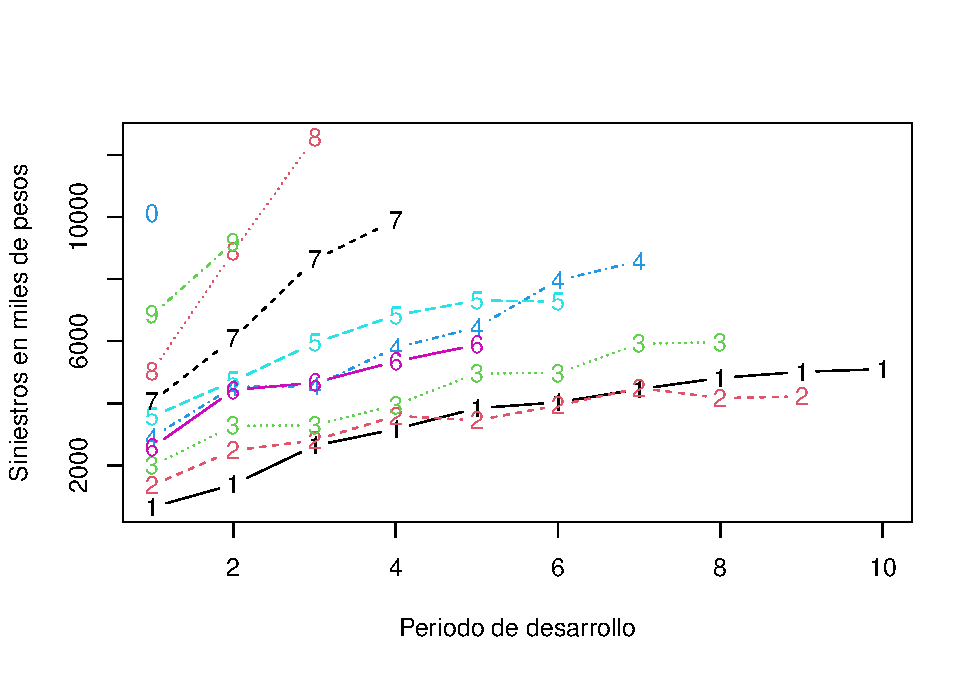
\includegraphics{informe_files/figure-latex/unnamed-chunk-4-1.pdf}
\caption{\label{triangle} Desarrollo de los reclamos por año y período.}
\end{figure}

\section{Chain-Ladder}\label{chain-ladder}

El objetivo de este trabajo es presentar distintos métodos para estimar
los siniestros incurridos que se tendrán pasado los años de desarrollo.
Y de esta manera obtener la reserva necesaria para hacer frente a lo que
será reclamado.

Una de las principales herramientas del Chain-Ladder son los factores de
desarrollo que se definiran más adelante. Se utilizan tanto en las
matrices de pagos acumulados como en la de siniestros incurridos, y es
el factor por el que los valores van creciendo de un período a otro. A
veces se utiliza un solo factor de desarrollo para todo el período de
desarrollo (ejemplo, para el crecimiento de los siniestros/pagos del
período 6 al 7, sin importar el año de ocurrencia, lo que sería columna
por columna) y a veces es de particular interés los factores
individuales, es decir, poder diferenciar tanto para el período de
desarrollo como al año de ocurrencia (celda por celda).

En primer lugar se presentará el método de \textbf{Chain-Ladder
clásico}, que utiliza la información del desarrollo de los reportes de
los siniestros durante los años posteriores a que hayan ocurrido para
predecir cómo se comportarán en el futuro, que en general, se suele
asumir que luego de terminado el último período de desarrollo, no habrá
nuevos reclamos y los costos no aumentarán. Luego, se presentará una
variación del método, que utiliza un modelo de regresión en función de
los años transcurridos a partir de los factores de desarrollos
observados, de esta manera, obtener mediante estimaciones un factor de
desarrollo mayor a 1 para el último período de desarrollo. Después se
presentará el método de \textbf{Mack Chain-Ladder}, que bajo ciertos
supuestos, obtiene una estimación de los desvíos de los siniestros a
futuros y de la reserva de IBNR. Por último se presentará el método de
\textbf{Munich Chain-Ladder} que utiliza un modelo de regresión y parte
de la correlación existente entre los siniestros incurridos y los pagos
acumulados.

\subsection{Chain Ladder `clásico'}\label{chain-ladder-cluxe1sico}

Uno de los métodos más utilizados es el de ``Chain Ladder'' (Escalera de
Cadena). A partir de la matriz que se puede ver en el cuadro
\ref{tabla1}, cálcula los factores de desarrollo, que miden el
crecimiento de los gastos por siniestro pasado los años. El factor de
desarrollo representa la proporción que aumentan el monto de los
siniestros incurridos entre dos períodos consecutivos (el factor de
desarrollo \(q_j\) representa el aumento de los siniestros incurridos
entre el período \(j\) y el \(j+1\)). Para el cálculo de este, se suma
todos los siniestros incurridos en el período \(j+1\), es decir
\(\sum_{i=1}^{n-j} X_{i,j+1}\) y se los divide entre la misma cantidad
de filas, del período anterior (\(j\)), es decir
\(\sum_{i=1}^{n-j} X_{i,j}\) de esta forma se obtiene: \[
\hat{q}_{j} = \frac{\sum_{i=1}^{n-j} X_{i,j+1}}{\sum_{i=1}^{n-j} X_{i,j}}
\] Obersevesé la figura \ref{captura1}, la cual representa la matriz de
los siniestros incrurridos,equivalente al cuadro \ref{tabla1}. En
sombreado las columnas del período 1 y 2 necesarias para cálcular
\(\hat{q}_{1}\).

\begin{figure}[ht]
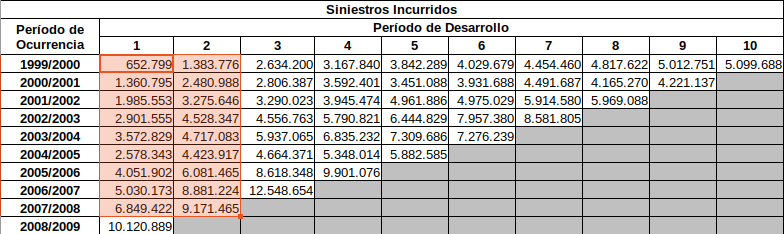
\includegraphics[width=1\linewidth]{imagenes/captura1} \caption{\label{captura1} En sombreado, las filas de la columna correspondiente al período de desarrollo 1 y 2, que se dividen para calcular el factor de desarrollo del período 1.}\label{fig:unnamed-chunk-5}
\end{figure}

Por otro lado, se define el \emph{factor de desarrollo acumulado},
\(Q_{j}\), que se obtiene de de manera iterativa, de la forma: \[
Q_{j-1} = q_{j-1}\cdot Q_{j}
\] En particular, para el último período de desarrollo se tiene, en
general, que \(Q_n = 1\) con \(n\) correspondiente al último período.

Una vez obtenidos los factores, se puede predecir los siniestros
incurridos para los valores por debajo de la diagonal de la manera: \[
X_{i,c_i +1} = X_{i,c_i} \cdot q_{c_i}
\] siendo \(i\) el período de ocurrencia, \(c_i\) es el último período
de desarrollo que se tiene información y \(q_{c_i}\) el factor de
desarrollo del período de desarrollo \(c_i\).

De forma inmediata, se puede obtener con los factores de desarrollo
acumulado el total a pagar y reservar por los siniestros ocurridos en el
año \(i\) (\(X_i\)) de la manera: \[
X_i = Q_{c_i} \cdot X_{i,c_i}
\] Que da el mismo resultado que hacer
\(X_i = X_{i,c_i} \cdot q_{c_i} \cdot \cdots \cdot q_{n}\), es decir,
predecir todos los valores de la fila por debajo de la diagonal, y
quedarnos con la última columna. Donde \(c_i = n-i+1\) y queda definida
la diagonal con todos los pares \((i,c_i)\).

Luego, denominamos a \(X_i\) como la \emph{pérdida esperada} por los
siniestros incurridos en el año \(i\). La reserva de \(IBNR_i\) del
período \(i\), es la reserva para los siniestros ocurridos en el año
\(i\) y que fueron denunciados en los años posteriores. Será calculada
como la diferencia entre la pérdida esperada, y el último período para
el que tenemos los pagos acumulados y reservados en la matriz de
siniestros incurridos (\(X_{i,c_i}\)) \[
IBNR_i = X_i - X_{i,c_i} 
\] Finalmente obtenemos el \(IBNR\) como la suma total de los \(IBNR_i\)
para cada período de ocurrencia: \[
IBNR = \sum_{i=1}^n IBNR_i = \sum_{i=1}^n X_i - X_{i,c_i} 
\]

El cuadro \ref{exhibit} representa un resúmen de los cálculos a realizar
para obtener el \(IBNR\), en la primer columna se representa el
\(X_{i,c_i}\), en la segunda el \(Q_i\), en la tercera \(X_i\) y en la
última el \(IBNR_i\).

\begin{table}[ht]
\centering
\caption{Cálculo del IBNR según el método clásico.} 
\label{exhibit}
\begingroup\fontsize{10pt}{10pt}\selectfont
\begin{tabular}{ccccc}
  \hline
 & Último siniestro incurrido & Factor de desarrollo acumulado & Pérdida Esperada & IBNR \\ 
  \hline
1999 & 5099688.00 & 1.00 & 5099688.00 & 0.00 \\ 
  2000 & 4221137.00 & 1.02 & 4292896.33 & 71759.33 \\ 
  2001 & 5969088.00 & 1.04 & 6237696.96 & 268608.96 \\ 
  2002 & 8581805.00 & 1.05 & 9028058.86 & 446253.86 \\ 
  2003 & 7276239.00 & 1.18 & 8585962.02 & 1309723.02 \\ 
  2004 & 5882585.00 & 1.28 & 7517943.63 & 1635358.63 \\ 
  2005 & 9901076.00 & 1.42 & 14069429.00 & 4168353.00 \\ 
  2006 & 12548654.00 & 1.69 & 21169579.30 & 8620925.30 \\ 
  2007 & 9171465.00 & 2.12 & 19489363.12 & 10317898.12 \\ 
  2008 & 10120889.00 & 3.30 & 33368571.03 & 23247682.03 \\ 
  Total & 78772626.00 &  & 128859188.25 & 50086562.25 \\ 
   \hline
\end{tabular}
\endgroup
\end{table}

En algunas ocasiones, la asignación de un valor \(Q_n=1\) para el último
período de desarrollo puede no ser lo mejor para la representación de la
realidad, de esta forma, se puede asignar un valor mayor a 1 para el
factor de desarrollo del último año, \(Q_n>1\), por ejemplo
\(Q_n=1,05\), cabe aclarar que los siguientes factores de desarrollo
quedaran determinados a partir de este primero.

\subsection{Chain Ladder con
regresión}\label{chain-ladder-con-regresiuxf3n}

Este modelo permite calcular el factor de desarrollo para \(Q_n\)
asumiendo una estructura de regresión para los factores de desarrollos
(simples) en función de los períodos de desarrollo. Si bien estos no
varían mucho a lo largo del tiempo, si se puede observar una estructura
de regresión lineal si hacemos el logaritmo del aumento proporcional
(\(q-1\)) de los siniestros incurridos en función de los períodos de
desarrollo \(Log(q-1) \sim \text{períodos de desarrollo}\). \[
Log(q_j -1) = \alpha + \beta\cdot j
\] siendo \(\alpha\) la ordenada en el origen, \(\beta\) la pendiente y
\(j\) el período de de desarrollo.

El cuadro \ref{factores1} representa los factores de desarrollo para
cada período, \(q_j\), de los siniestros incurridos presentados en el
cuadro \ref{tabla1}.

\begin{table}[ht]
\centering
\caption{Factores de desarrollo de los sinisestros incurridos.} 
\label{factores1}
\begin{tabular}{cc}
  \hline
 & Factores de desarrollo \\ 
  \hline
1 & 1.551 \\ 
  2 & 1.260 \\ 
  3 & 1.187 \\ 
  4 & 1.112 \\ 
  5 & 1.083 \\ 
  6 & 1.122 \\ 
  7 & 1.006 \\ 
  8 & 1.028 \\ 
  9 & 1.017 \\ 
   \hline
\end{tabular}
\end{table}

Para modelar una regresión lineal de la forma
\(Log(q_j -1) = \alpha + \beta\cdot j\), es necesario haber calculado
los factores de desarrollo. Previamente chequendo si para el gráfico de
dispersión de los datos corresponde el modelo de regresión lineal. Una
vez obtenidos los \(q_j\) se modela. La figura \ref{regresion}
representa el resultado de la misma.

\begin{figure}[H]
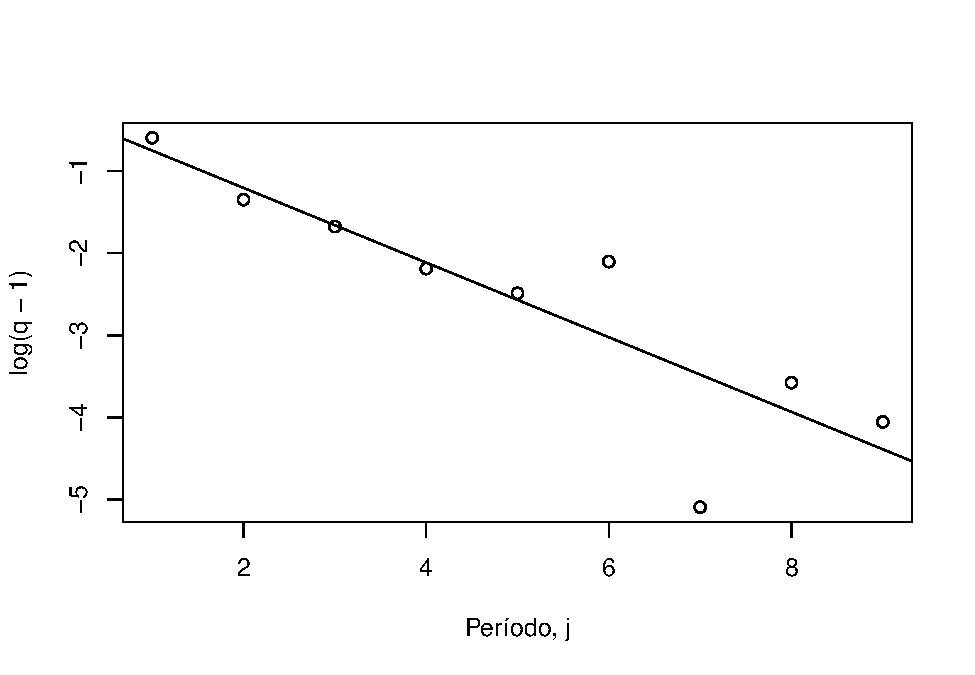
\includegraphics[width=1\linewidth]{informe_files/figure-latex/unnamed-chunk-9-1} \caption{\label{regresion} Extrapolación Log-lineal de los factores año a año.}\label{fig:unnamed-chunk-9}
\end{figure}

Luego, se sugiere extrapolar los datos para 100 períodos de desarrollo,
y se puede observar que el \(Log(q_j -1)\) empieza a converger cuando
\(j\) aumenta. De esta forma podemos obtener una estimación para
\(Q_n\), podemos calcular como:
\[\hat{Q_n} = \prod_{j\geq n} \hat{q_{j}} \] De esta forma para los
siniestros incurridos que venimos viendo, se obtiene
\(\hat{Q_n} = 1.021795\).

La figura \ref{regresion2} representa la extrapolación a 100 períodos de
desarrollo.

\begin{figure}
\subfloat[\label{reg1} 109 períodos de desarrollo.\label{fig:unnamed-chunk-10-1}]{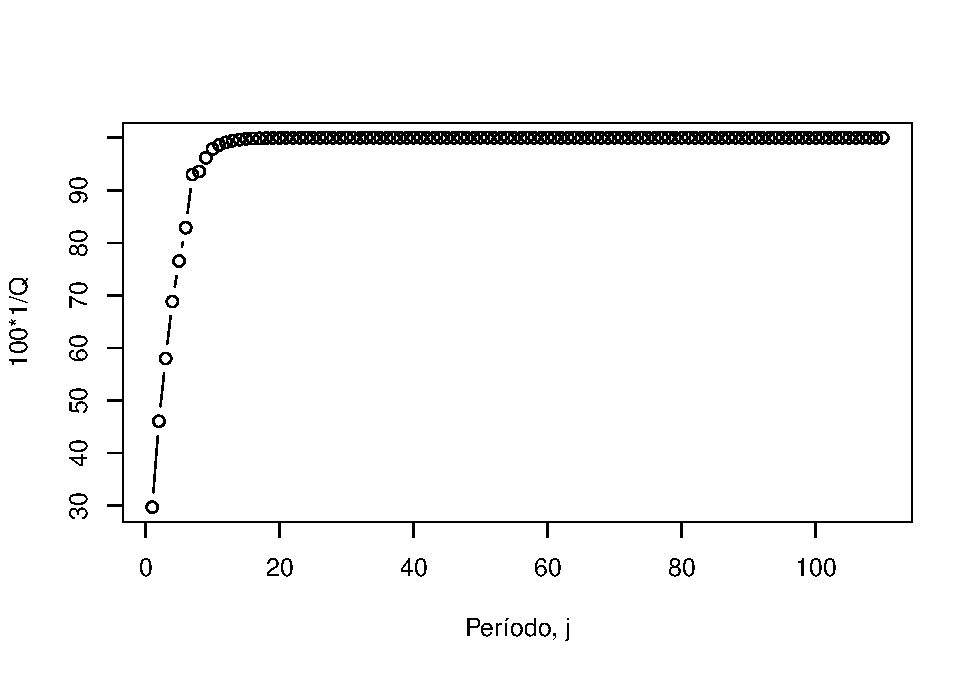
\includegraphics[width=0.5\linewidth]{informe_files/figure-latex/unnamed-chunk-10-1} }\subfloat[\label{reg2} Primeros 19 períodos de desarrollo.\label{fig:unnamed-chunk-10-2}]{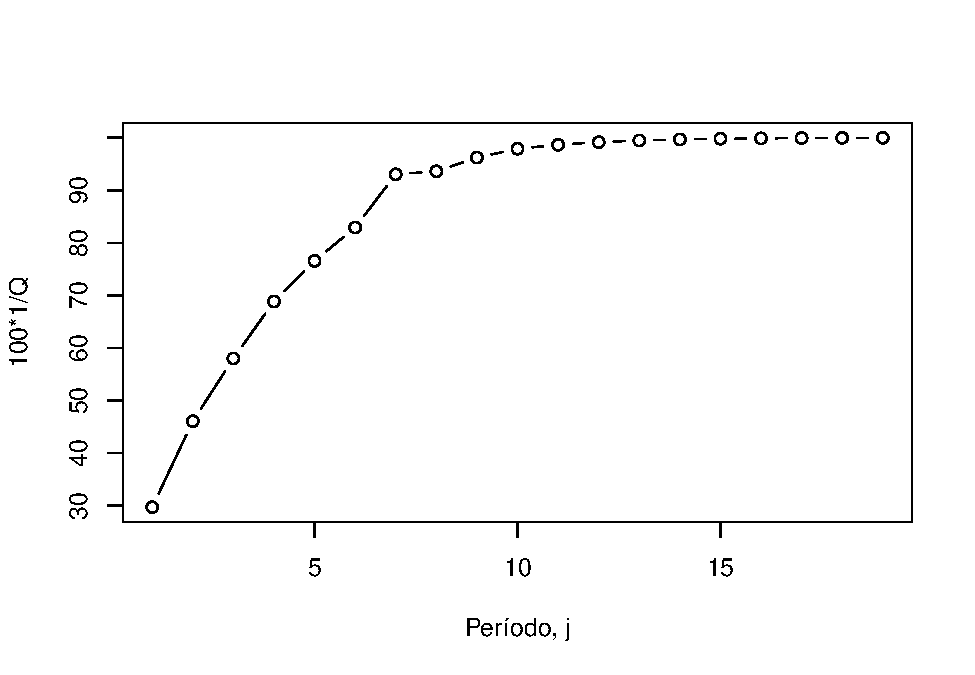
\includegraphics[width=0.5\linewidth]{informe_files/figure-latex/unnamed-chunk-10-2} }\caption{\label{regresion2} Patrón de desarrollo de reclamaciones esperado.}\label{fig:unnamed-chunk-10}
\end{figure}

Nuestros factores de desarrollo serán los obtenidos normalmente hasta el
momento \(n-1=9\) y para \(q_n=q_{10}\) se le asigna el valor de
\(\hat{Q_n}\) calculado anteriormente, que para el último período de
desarrollo era válida la equivalencia.

De esta forma, se hace el análogo al cuadro \ref{exhibit} y se cálcula
nuevamente el \(IBNR\) con este método, observesé los resultados en el
cuadro \ref{exhibit2}.

\begin{table}[ht]
\centering
\caption{Cálculo del IBNR según el método con regresión.} 
\label{exhibit2}
\begingroup\fontsize{10pt}{10pt}\selectfont
\begin{tabular}{ccccc}
  \hline
 & Último siniestro incurrido & Factor de desarrollo acumulado & Pérdida Esperada & IBNR \\ 
  \hline
1999 & 5099688.000 & 1.022 & 5211881.136 & 112193.136 \\ 
  2000 & 4221137.000 & 1.040 & 4389982.480 & 168845.480 \\ 
  2001 & 5969088.000 & 1.069 & 6380955.072 & 411867.072 \\ 
  2002 & 8581805.000 & 1.075 & 9225440.375 & 643635.375 \\ 
  2003 & 7276239.000 & 1.206 & 8775144.234 & 1498905.234 \\ 
  2004 & 5882585.000 & 1.306 & 7682656.010 & 1800071.010 \\ 
  2005 & 9901076.000 & 1.453 & 14386263.428 & 4485187.428 \\ 
  2006 & 12548654.000 & 1.724 & 21633879.496 & 9085225.496 \\ 
  2007 & 9171465.000 & 2.172 & 19920421.980 & 10748956.980 \\ 
  2008 & 10120889.000 & 3.368 & 34087154.152 & 23966265.152 \\ 
  Total & 78772626.000 &  & 131693778.363 & 52921152.363 \\ 
   \hline
\end{tabular}
\endgroup
\end{table}

Se observa que al asignarle un factor de desarrollo acumulado mayor a 1
para el último período de desarrollo, se obtiene que las reservas por
IBNR aumentan aproximadamente en \$3.000.000 respecto al método clásico
representado en el cuadro \ref{exhibit}, este monto representa
aproximadamente un aumento del \%5 en las reservas. Esto se traduce en
menores ganancias para la compañia aseguradora pero permite estar mas
cubierto frente a acontecimientos siniestrales ocurridos pero no
reportados.

\section{Mack Chain-Ladder}\label{mack-chain-ladder}

Thomas Mack publica en 1993 un método para obtener estimaciones de los
errores estándar de las estimaciones de pérdida esperada, y por
consecuencia del IBNR, se puede aplicar tanto en la matriz triangular de
pérdida acumulada como en la matriz triangular de siniestros incurridos,
y es un método para predecir el triángulo inferior faltante de la
matriz, es decir, los siniestros incurridos a futuro de cada año de
ocurrencia para cada período de desarrollo.

Para predecir los siniestros incurridos a futuro \(X_{i,j}\) con
\(j>n-i+1\) se asume:

\begin{itemize}

\item $\mathbb{E}(q_{i,j}|X_{i,1},\ldots,X_{i,j}) = q_j$ con $q_{i,j} = \frac{X_{i,j+1}}{X_{i,j}}$

\item $\mathbb{V}(q_{i.j}|X_{i,1},\ldots,X_{i,j}) = \frac{\sigma^2_j}{w_{i,j}X_{i,j}^\alpha} $

\item $\{ X_{i,1},\ldots,X_{i,n} \}, \{X_{k,1},\ldots,X_{k,n}\}$ son independientes del período de origen ($i \neq k$)

\end{itemize}

Con \(w_{i,j} \in [0;1]\) y \(\alpha \in \{0,1,2\}\), se obtienen
estimaciones insesgadas de las pérdidas esperadas y de las reservas de
IBNR junto a los errores estándar y el coeficiente de variación.

Luego, a partir de la fórmula del error cuadrático medio,
\(ECM(\hat{X}_{i,n})=\mathbb{E}((\hat{X}_{i,n}-X_{i,n})^2|X_{i,1}\ldots,X_{i,n-i+1})=\mathbb{V}(\hat{X}_{i,n}) + (\mathbb{E}(X_{i,n}|X_{i,1}\ldots,X_{i,n-i+1})-\hat{X}_{i,n})^2\)
se podrá calcular el error cuadrático medio como la suma de los errores
estocásticos y el error de estimación y se necesitará una fórmula para
la varianza.

Se puede notar que el factor de desarrollo \(q_j\) es el promedio
ponderado de los factores \(q_{i,j}=X_{i,j+1}/X_{i,j}\), por lo que la
varianza de \(X_{i,j+1}/X_{i,j}\) (dado los siniestros hasta el período
de desarrollo j) es inversamente proporcional a \(X_{i,j}\), donde se
asume que todos los siniestros incurridos pesan igual y \(\alpha=1\) en
las condiciones planteadas anteriormente.

\[
\mathbb{V}(X_{i,j+1}|X_{i,1},\ldots,X_{i,j}) = X_{i,j}\cdot \sigma_j^2
\] Donde \(\sigma_j^2\) es un parámetro desconocido que debe ser
estimado, y es la varianza implícita bajo el método de `Chain Ladder'.
Por lo que la varianza estimada será la suma de los errores al cuadrado
ponderados de la estimación de los factores de desarrollo año a año.

\[
\hat{\sigma_j}^2 = \frac{1}{n-j-1}\cdot \sum_{i=1}^{n-j} X_{i,j}\left( \frac{X_{i,j+1}}{X_{i,j}} - \hat{q_j} \right)^2=\frac{1}{n-j-1}\cdot \sum_{i=1}^{n-j} X_{i,j}\left( q_{i,j} - \hat{q_j} \right)^2
\]

Siendo \(\hat{\sigma_j}^2\) un estimador insesgado para
\(1 \leq j \leq n-2\), obteniendo una estimación del desvío al hacer la
raíz. Para estimar \(\sigma_{n-1}\) , si se tiene que
\(\hat{q}_{n-1}=1\) se puede utilizar \(\sigma_{n-1}=0\) ya que se asume
que el desarrollo de los siniestros termina en el tiempo \(n-1\), de lo
contrario se puede extrapolar utilizando la reducción exponencial de los
desvíos de forma tal que \(\hat{\sigma}_{n-1}\) cumpla con la razón.

\[
\frac{\hat{\sigma}_{n-3}}{\hat{\sigma}_{n-2}} = \frac{\hat{\sigma}_{n-2}}{\hat{\sigma}_{n-1}}
\]

\[
\hat{\sigma}_{n-1} = \frac{\hat{\sigma}_{n-2}^2}{\hat{\sigma}_{n-3}}
\]

Siendo \(R_i\) las reservas de IBNR del año \(i\), estas son calculadas
como \(R_i = X_{i,n} - X_{i,n-i+1}\) y estimadas de la forma
\(\hat{R}_i = \hat{X}_{i,n} - X_{i,n-i+1}\) donde el total de los costos
incurridos del año \(i\) son estimados a través de los factores de
desarrollo, ya sea calculando el total para todos los años de desarrollo
con los factores año a año, o a través del factor de desarrollo
acumulado \(\hat{X}_{i,n} = Q_{n-i+1}\cdot X_{i,n-i+1}\). Luego, como la
única parte aleatoria de \(\hat{R}_i\) es \(\hat{X}_{i,n}\) el
\(ECM(\hat{R}_i) = ECM(\hat{X}_{i,n})\)

\[
\widehat{ECM}(\hat{R}_i) = \hat{X}_{i,n}^2 \sum_{j=n-i+1}^{n-1} \frac{\hat{\sigma_j}^2}{\hat{q}_j}\left( \frac{1}{\hat{X}_{i,j}} - \frac{1}{\sum_{l=1}^{I-j}X_{l,j}} \right)
\]

La función \texttt{MackChainLadder} del paquete \texttt{ChainLadder} nos
da una tabla con las reservas de IBNR para cada año, su desvío y su
coeficiente de variación, y las mismas medidas para el total, teniendo
especial atentción de que el desvío del total no es igual a la suma del
desvío, nos muestra la última pérdida obtenida, la última pérdida
esperada, la relación entre estas, la reserva de IBNR, el desvío y el
coeficiente de variación.

\begin{table}[ht]
\centering
\caption{Estimaciones mediante Método Mack Chain-Ladder por año de Ocurrencia} 
\label{origin2}
\begingroup\fontsize{10pt}{10pt}\selectfont
\begin{tabular}{ccccccc}
  \hline
 & Latest & Dev.To.Date & Ultimate & IBNR & Mack.S.E & CV(IBNR) \\ 
  \hline
1999 & 5099688.00 & 1.00 & 5099688.00 & 0.00 & 0.00 &  \\ 
  2000 & 4221137.00 & 0.98 & 4294344.90 & 73207.90 & 158102.19 & 2.16 \\ 
  2001 & 5969088.00 & 0.96 & 6242289.13 & 273201.13 & 246430.13 & 0.90 \\ 
  2002 & 8581805.00 & 0.95 & 9029697.31 & 447892.31 & 708612.58 & 1.58 \\ 
  2003 & 7276239.00 & 0.85 & 8589919.40 & 1313680.40 & 782964.48 & 0.60 \\ 
  2004 & 5882585.00 & 0.78 & 7521436.22 & 1638851.22 & 1070034.24 & 0.65 \\ 
  2005 & 9901076.00 & 0.70 & 14077508.98 & 4176432.98 & 1880770.51 & 0.45 \\ 
  2006 & 12548654.00 & 0.59 & 21175489.41 & 8626835.41 & 2602113.44 & 0.30 \\ 
  2007 & 9171465.00 & 0.47 & 19492933.42 & 10321468.42 & 3717510.05 & 0.36 \\ 
  2008 & 10120889.00 & 0.30 & 33356395.46 & 23235506.46 & 6120205.09 & 0.26 \\ 
   \hline
\end{tabular}
\endgroup
\end{table}

\begin{table}[ht]
\centering
\caption{Estimaciones mediante Método Mack Chain-Ladder para el total} 
\label{total2}
\begingroup\fontsize{10pt}{10pt}\selectfont
\begin{tabular}{cc}
  \hline
 & Totals \\ 
  \hline
Latest: & 78772626.00 \\ 
  Dev: & 0.61 \\ 
  Ultimate: & 128879702.24 \\ 
  IBNR: & 50107076.24 \\ 
  Mack S.E.: & 11156939.54 \\ 
  CV(IBNR): & 0.22 \\ 
   \hline
\end{tabular}
\endgroup
\end{table}

También se puede acceder a los factores mediante \texttt{mackTRI\$f}
(Cuadro \ref{factores}), o a la matriz completa con la estimación de los
siniestros incurridos en los años siguientes mediante
\texttt{mackTRI\$FullTriangle} (Cuadro \ref{fulltriangle}).

\begin{table}[ht]
\centering
\caption{Factores de desarrollo} 
\label{factores}
\begin{tabular}{cc}
  \hline
 & Factores de desarrollo \\ 
  \hline
1 & 1.551 \\ 
  2 & 1.260 \\ 
  3 & 1.187 \\ 
  4 & 1.112 \\ 
  5 & 1.083 \\ 
  6 & 1.122 \\ 
  7 & 1.006 \\ 
  8 & 1.028 \\ 
  9 & 1.017 \\ 
  10 & 1.000 \\ 
   \hline
\end{tabular}
\end{table}

\begin{table}[ht]
\centering
\caption{Matriz Completa con la estimación de los Siniestros Incurridos a futuro} 
\label{fulltriangle}
\begingroup\fontsize{8.2pt}{10pt}\selectfont
\begin{tabular}{lcccccccccc}
  \hline
 & 1 & 2 & 3 & 4 & 5 & 6 & 7 & 8 & 9 & 10 \\ 
  \hline
1999 & 652799 & 1360795 & 1985553 & 2901555 & 3572829 & 2578343 & 4051902 & 5030173 & 6849422 & 10120889 \\ 
  2000 & 1383776 & 2480988 & 3275646 & 4528347 & 4717083 & 4423917 & 6081465 & 8881224 & 9171465 & 15694252 \\ 
  2001 & 2634200 & 2806387 & 3290023 & 4556763 & 5937065 & 4664371 & 8618348 & 12548654 & 11551567 & 19767093 \\ 
  2002 & 3167840 & 3592401 & 3945474 & 5790821 & 6835232 & 5348014 & 9901076 & 14893269 & 13709884 & 23460415 \\ 
  2003 & 3842289 & 3451088 & 4961886 & 6444829 & 7309686 & 5882585 & 11010150 & 16561547 & 15245604 & 26088346 \\ 
  2004 & 4029679 & 3931688 & 4975029 & 7957380 & 7276239 & 6371162 & 11924596 & 17937063 & 16511825 & 28255109 \\ 
  2005 & 4454460 & 4491687 & 5914580 & 8581805 & 8163841 & 7148357 & 13379234 & 20125140 & 18526042 & 31701847 \\ 
  2006 & 4817622 & 4165270 & 5969088 & 8634502 & 8213971 & 7192252 & 13461390 & 20248719 & 18639802 & 31896514 \\ 
  2007 & 5012751 & 4221137 & 6135874 & 8875763 & 8443483 & 7393214 & 13837522 & 20814500 & 19160627 & 32787752 \\ 
  2008 & 5099688 & 4294345 & 6242289 & 9029697 & 8589919 & 7521436 & 14077509 & 21175489 & 19492933 & 33356395 \\ 
   \hline
\end{tabular}
\endgroup
\end{table}

La función \texttt{plot} recibe como argumento un objeto del tipo
\texttt{MackChainLadder} y genera graficos con las estimaciones de los
siniestros incurridos a futuro y un intervalo de confianza así como
información sobre los residuos estandarizados.

\begin{figure}
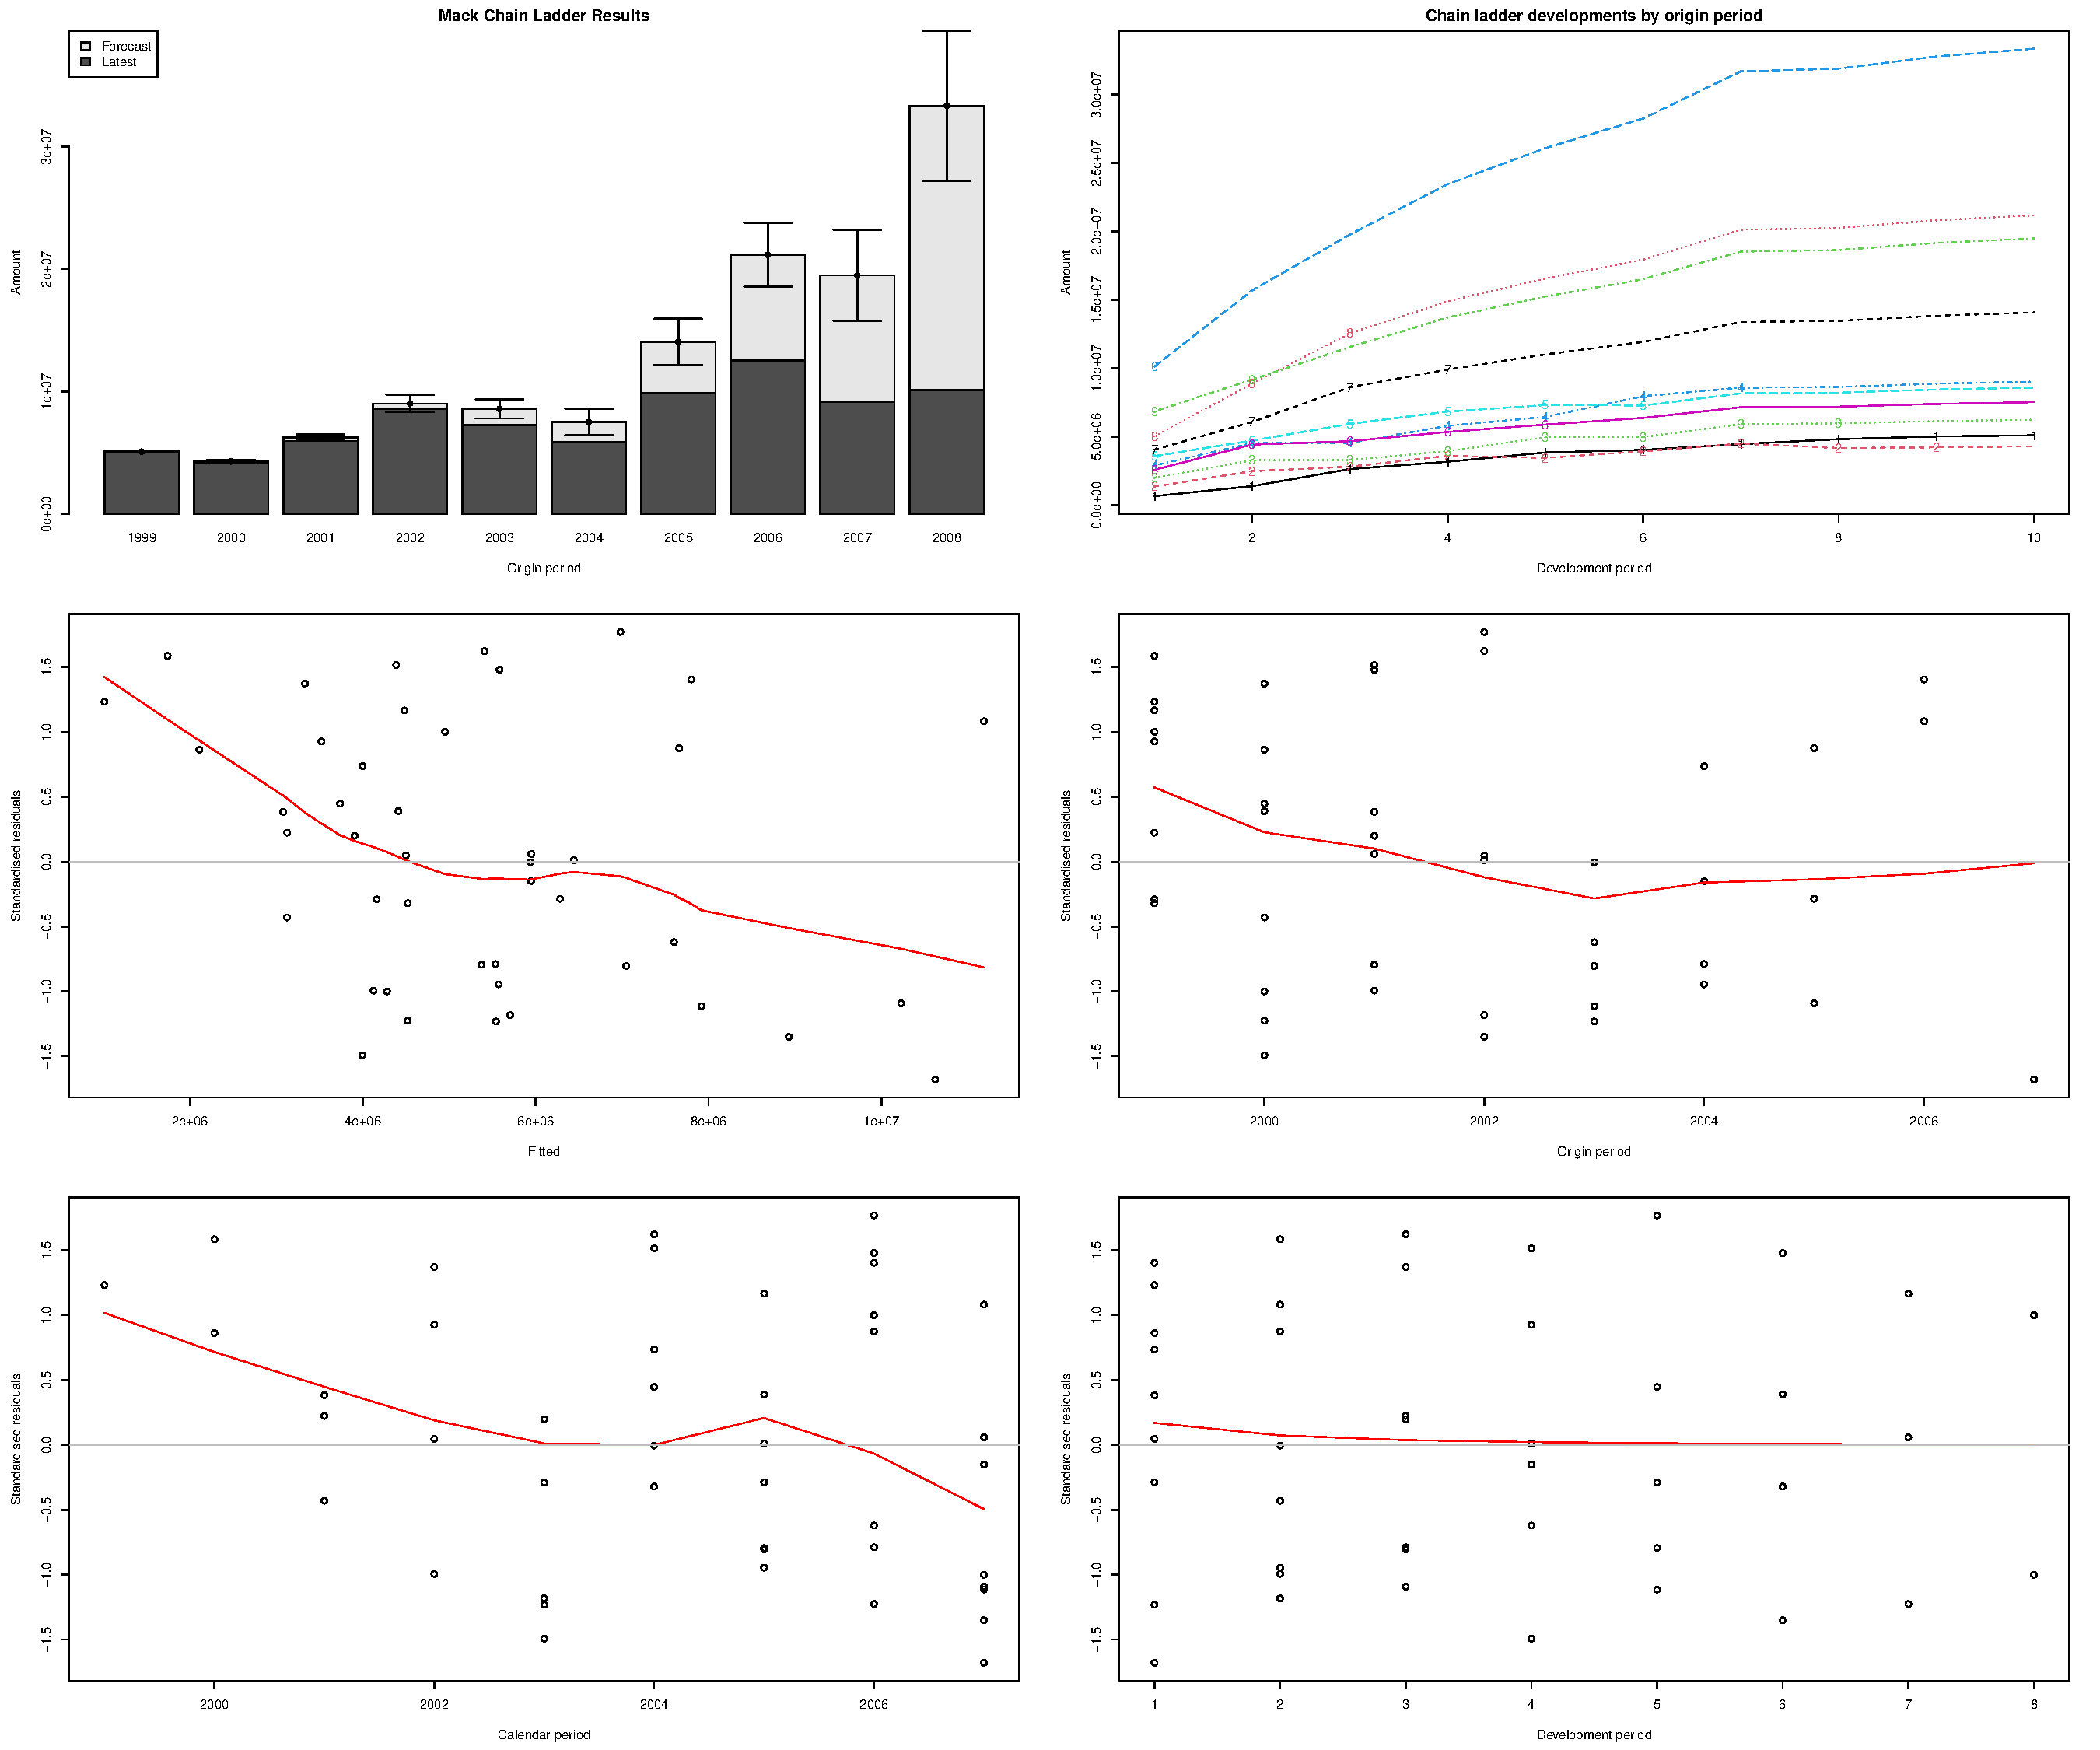
\includegraphics[width=1\linewidth]{informe_files/figure-latex/unnamed-chunk-18-1} \caption{Gráfico estandar para objetos MackChain-Ladder}\label{fig:unnamed-chunk-18}
\end{figure}

También se puede graficar la predicción del desarrollo de los siniestros
incurridos a futuro junto a una medida de la dispersión, separado por
cada año de ocurrencia, se puede notar que para años de ocurrencia más
reciente, para los cuáles se requiere estimar más valores, el intervalo
de confianza empieza en períodos de desarrollo anteriores, y tiene mayor
amplitud.

\begin{figure}
\centering
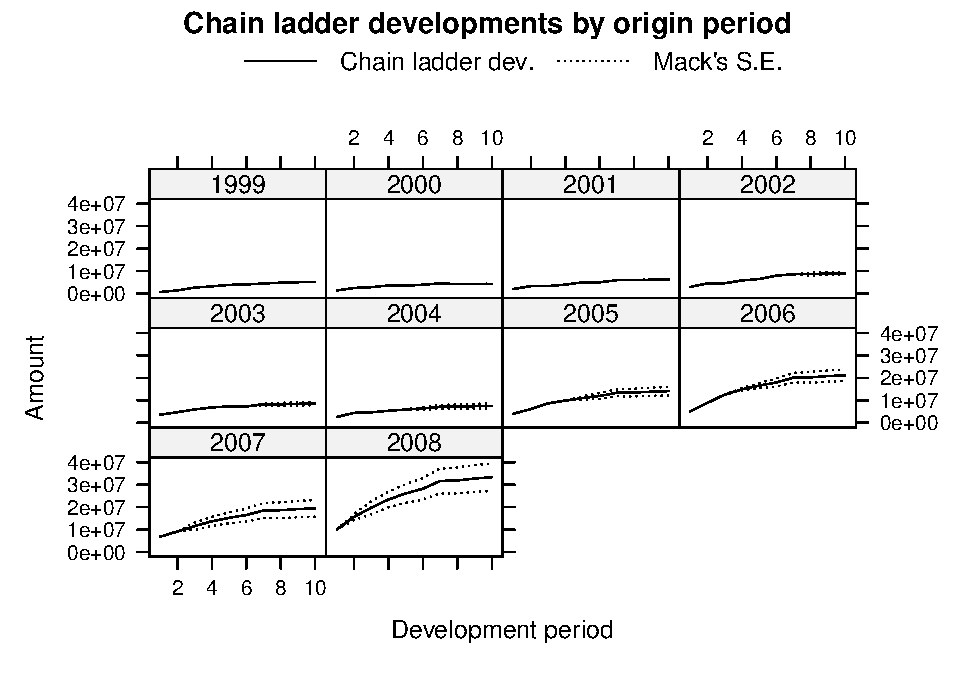
\includegraphics{informe_files/figure-latex/unnamed-chunk-19-1.pdf}
\caption{lattice = TRUE para obtener la estimación del desarrollo para
cada año de ocurrencia}
\end{figure}

\newpage

\section{Munich Chain Ladder}\label{munich-chain-ladder}

El método de Munich utiliza la correlación positiva entre el triángulo
de siniestros incurridos y el triángulo de siniestros pagados acumulados
para proyectar los futuros pagos. Como hasta ahora se venía trabajando
con el triángulo de siniestros incurridos, ahora se debe agregar el
triángulo de pagos acumulados.

Llamando \emph{I} a la matriz de siniestros incurridos y \emph{P} a la
matriz de siniestros pagados acumulados, se halla la matriz \(P/I\)
calculada como la división de celda a celda de la matriz \emph{P} entre
la matriz \emph{I}, y representa la fracción de los siniestros
incurridos que ya están pago de cada año ocurrencia durante los períodos
de desarrollo. Donde se suele observar que a medida que hay más períodos
de desarrollo la mayoría de los siniestros han sido pagados.

\begin{table}[ht]
\centering
\caption{Proporción de siniestros incurridos que han sido pagos en cada período de desarrollo.} 
\label{tabla2}
\begingroup\fontsize{11.5pt}{10pt}\selectfont
\begin{tabular}{ccccccccccc}
  \hline
 & 1 & 2 & 3 & 4 & 5 & 6 & 7 & 8 & 9 & 10 \\ 
  \hline
1999 & 0.5712 & 0.4191 & 0.2374 & 0.2043 & 0.2524 & 0.3934 & 0.5571 & 0.6733 & 0.8434 & 0.8644 \\ 
  2000 & 0.2671 & 0.2708 & 0.2546 & 0.2058 & 0.2168 & 0.2695 & 0.4919 & 0.7259 & 0.7843 &  \\ 
  2001 & 0.3263 & 0.3150 & 0.3936 & 0.4187 & 0.4143 & 0.4693 & 0.4024 & 0.3657 &  &  \\ 
  2002 & 0.1413 & 0.2445 & 0.3226 & 0.2988 & 0.3824 & 0.5337 & 0.5969 &  &  &  \\ 
  2003 & 0.2329 & 0.3176 & 0.2790 & 0.2980 & 0.3529 & 0.3592 &  &  &  &  \\ 
  2004 & 0.3728 & 0.3429 & 0.4024 & 0.4045 & 0.3816 &  &  &  &  &  \\ 
  2005 & 0.5250 & 0.5667 & 0.5095 & 0.4520 &  &  &  &  &  &  \\ 
  2006 & 0.4937 & 0.4846 & 0.4755 &  &  &  &  &  &  &  \\ 
  2007 & 0.4634 & 0.5191 &  &  &  &  &  &  &  &  \\ 
  2008 & 0.4818 &  &  &  &  &  &  &  &  &  \\ 
   \hline
\end{tabular}
\endgroup
\end{table}

\subsection{Problemas del Chain-Ladder por separado
(SCL)}\label{problemas-del-chain-ladder-por-separado-scl}

Formalmente, se tiene que \((P/I)_{i,j} = P_{i,j}/I_{i,j}\), luego,
mediante los métodos vistos antes de Chain Ladder se puede estimar los
valores faltantes de ambas matrices con los factores de desarrollo año a
año a partir de la diagonal inversa, obteniendo el resultado de los
ratios si se hace Chain-Ladder por separado (Método SCL).

\begin{figure}
\subfloat[\label{graf1} Valores observados.\label{fig:unnamed-chunk-23-1}]{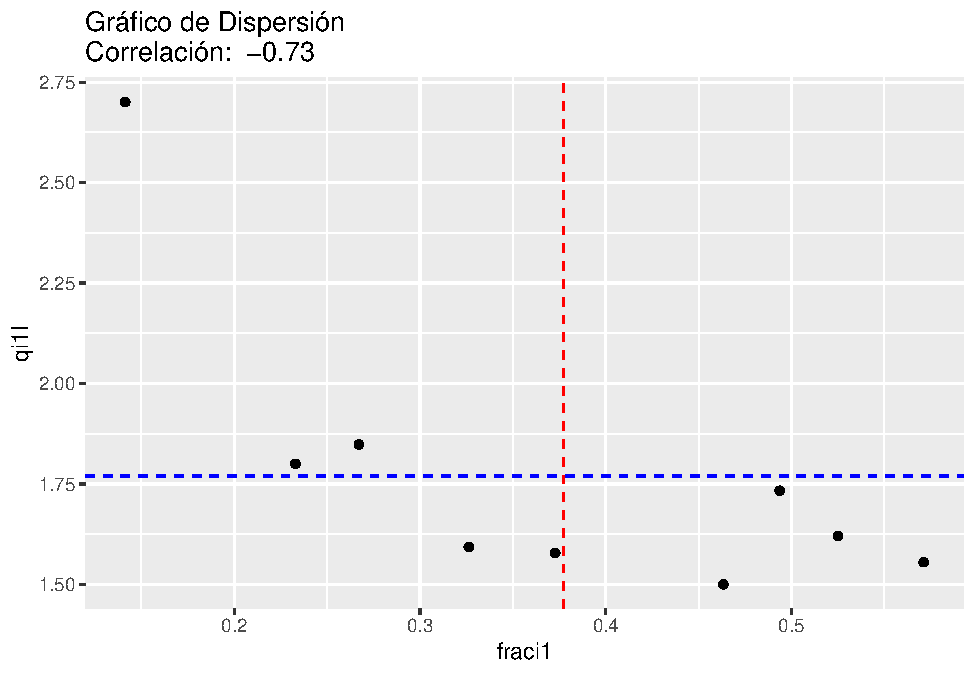
\includegraphics[width=0.5\linewidth]{informe_files/figure-latex/unnamed-chunk-23-1} }\subfloat[\label{graf2} Valores observados y proyectados.\label{fig:unnamed-chunk-23-2}]{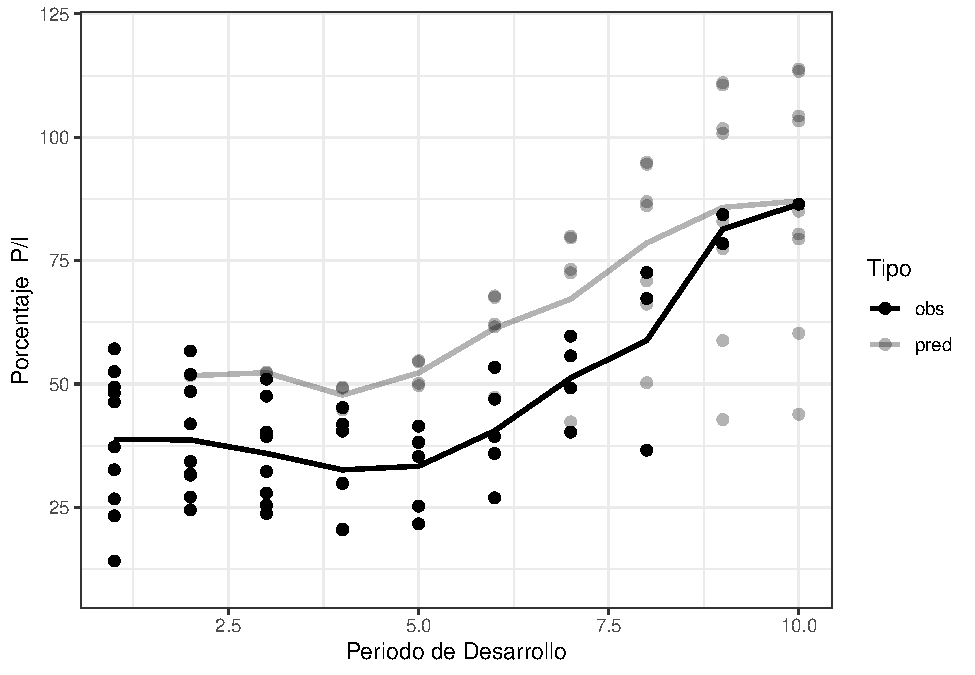
\includegraphics[width=0.5\linewidth]{informe_files/figure-latex/unnamed-chunk-23-2} }\caption{\label{graficos} Ratio P/I en 100\% con recta que une las medias por período de desarrollo}\label{fig:unnamed-chunk-23}
\end{figure}

Se puede notar en la figura \ref{graf2} que para los valores proyectados
en las dos matrices por separado a partir de cierto período de
desarrollo se tiene que los siniestros pagados significan una proporción
mayor a 1 que los siniestros incurridos, este error se da debido a que
se aplicó el método de Chain-Ladder por separado a ambos triángulos
(SCL) y no se tuvo en cuenta la estructura de correlación entre ambos
triángulos.

Para concluir el principal resultado de este método, se debe hacer
cuentas con los factores de desarrollo y las proyecciones tanto en la
matriz de pagos acomulados como la de siniestros incurridos. Para esto
define el promedio de los ratios en el período de desarrollo t:

\[
(P/I)_t := \frac{\sum_{j=1}^n P_{j,t}}{\sum_{j=1}^n I_{j,t}} = \frac{1}{\sum_{j=1}^n I_{j,t}}\cdot \sum_{j=1}^n I_{j,t}\cdot (P/I)_{j,t}
\]

Y luego, recordando que \(c_i:n-i+1\) es el último período de desarrollo
del que se tiene información para los siniestros, tanto los pagados
acumulados como los incurridos en el año \(i\) y se puede observar que
los pares \((i,c_i)\) son los índices de la diagonal invertida de las
matrices. Observando que para el año \(i\), los valores de \(P_{i,t}\) y
\(I_{i,t}\) son proyecciones para \(t>c_i\) se tiene que el ratio
\((P/I)_{i,t}\) se calcula

\[
(P/I)_{i,t} = \frac{P_{i,t}}{I_{i,t}} = \frac{P_{i,c_i}\cdot q_{c_i}^P \cdot \ldots \cdot q_{t-1}^P}{I_{i,c_i}\cdot q_{c_i}^I \cdot \ldots \cdot q_{t-1}^I}
\]

A partir de las fórmulas de los factores de desarrollo, se nota que para
\(t>c_i\):

\[
(P/I)_{i,t} = \frac{P_{i.c_i}\cdot \frac{\sum_{j=1}^n P_{j,t}}{\sum_{j=1}^n P_{j,c_i}}}{I_{i.c_i}\cdot \frac{\sum_{j=1}^n I_{j,t}}{\sum_{j=1}^n I_{j,c_i}}}
\] Y reordenando se tiene la siguiente relación para los ratios
proyectados mediante la aplicación de Chain-Ladder por separado:

\[
\frac{(P/I)_{i,t}}{(P/I)_t} = \frac{(P/I)_{i,c_i}}{(P/I)_{c_i}}
\]

Que indica que para cada año de accidente, el ratio de \((P/I)_{i,t}\)
con el \((P/I)_t\) promedio en el período de desarrollo t, debe cumplir
la misma relación que en el período \(c_i\), y esto se ve claramente en
el gráfico \ref{graf2} cuando se hace Chain-Ladder por separado siendo
la principal debilidad de este método.

\subsection{Modelado con Munich
Chain-Ladder}\label{modelado-con-munich-chain-ladder}

El modelo de Munich Chain-Ladder incorpora la correlación entre la
matriz de pagos acumulados \(P\) y la de siniestros incurridos \(I\).
Vemos que la correlación entre los factores de desarrollo para cada año
de ocurrencia del primer período de desarrollo de la matriz de pagos
acumulados, es decir, el vector de \(q_{i,1}^P\)
\(\forall i = \{1,2,\ldots,10\}\) respecto a los ratios \((P/I)_{i,1}\)
es de \(-0.7278\).

\begin{figure}

{\centering 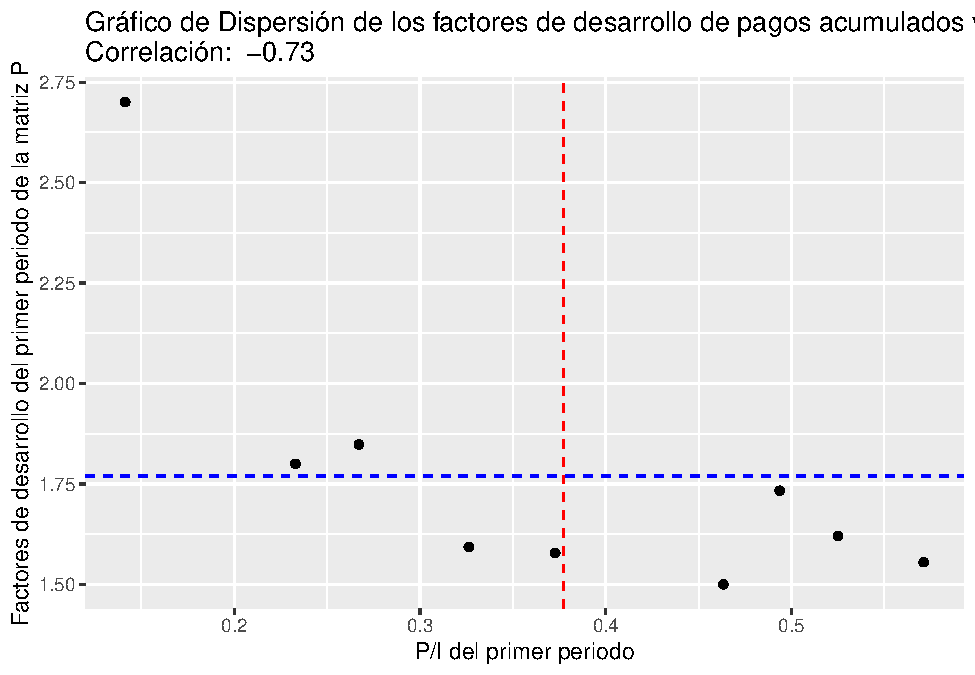
\includegraphics[width=0.8\linewidth]{informe_files/figure-latex/unnamed-chunk-25-1} 

}

\caption{\label{reg1_1} Gráfico de Puntos de Ratios P/I y Factores de desarrollo de la matriz de pagos acumulados para el primer período}\label{fig:unnamed-chunk-25}
\end{figure}

Y por otro lado, haciendo lo mismo para los factores de desarrollo
individuales del primer período de la matriz de siniestros incurridos y
los ratios del primer período de desarrollo se tiene una correlación
positiva más débil de \(0.3572\)

\begin{figure}

{\centering 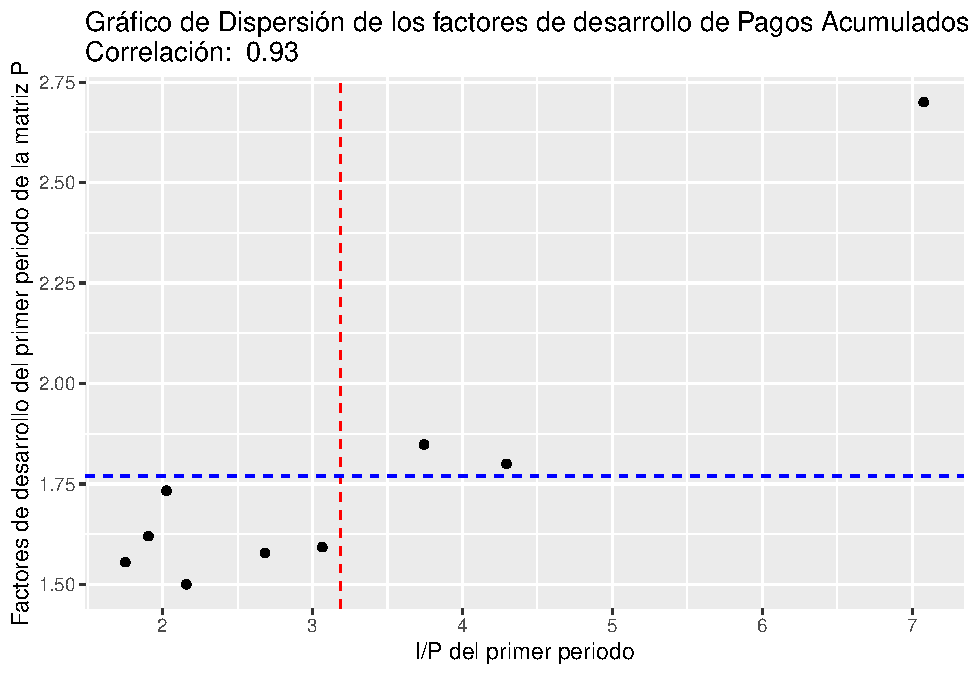
\includegraphics[width=0.8\linewidth]{informe_files/figure-latex/unnamed-chunk-27-1} 

}

\caption{\label{reg2_2} Gráfico de Puntos de Ratios P/I y Factores de desarrollo de la matriz de siniestros incurridos para el primer período}\label{fig:unnamed-chunk-27}
\end{figure}

Parece ser que uno de los problemas principales de hacer SCL es asumir
un factor igual para todos los años de ocurrencia, dado un período de
desarrollo y se nota que estos factores depende de los ratios \((P/I)\).

También es claro que con el correr de los períodos de desarrollo se
tendrán menos puntos en nuestro gráfico, y los resultados serán menos
consistentes, y además, los factores de desarrollo individuales para
cada año deben ser ajustados tanto para la matriz de pagos acumulados
como la de siniestros incurridos, pero la pregunta es en que medida cada
uno, esto expresa la idea básica para resolver el problema del método
SCL.

Siendo que para cada período de desarrollo se tiene un gráfico de puntos
como el anterior, pero cada vez con menos puntos, la idea es hacer una
regresión lineal en cada caso, y estimar el factor de desarrollo para
cada \((P/I)\), y de esta forma se puede predecir la parte restante de
la matriz. Por ejemplo, para el factor de desarrollo individual
\(q_{1,10}\) que no se tiene valores de la columna siguiente del
triángulo para calcularlo, se puede predecir con la regresión a partir
del valor \((P/I)_{1,10}\)

El método de Munich Chain-Ladder también incorpora los ratios
\((I/P)=1/(P/I)\), y la regresión de los factores de desarrollo de los
pagos acumulados se hace respecto a este ratio.

\begin{figure}

{\centering 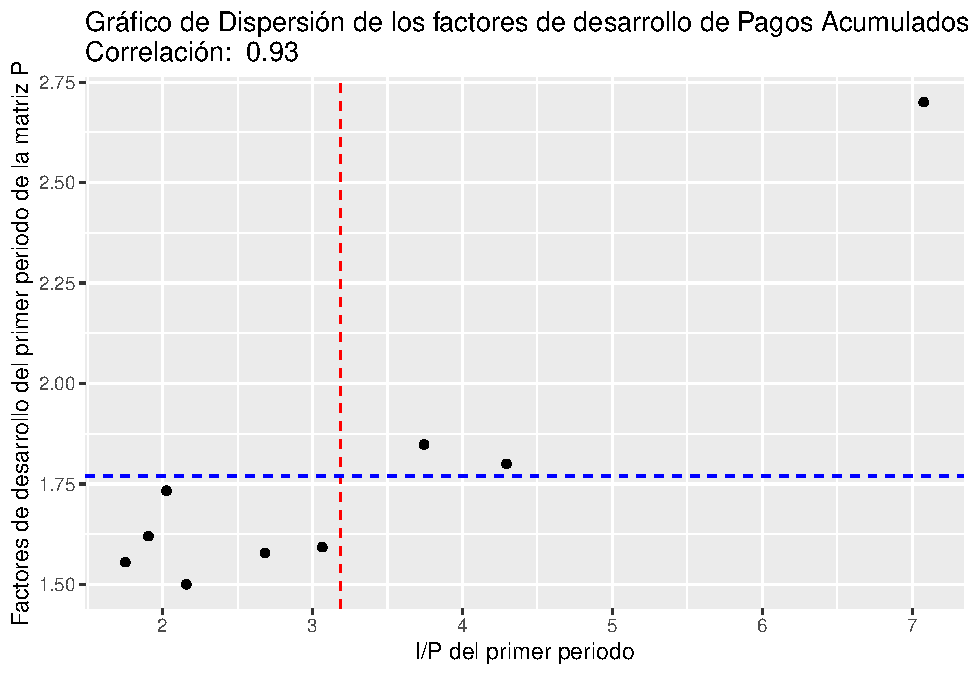
\includegraphics[width=0.8\linewidth]{informe_files/figure-latex/unnamed-chunk-28-1} 

}

\caption{\label{reg3} Gráfico de Puntos de Ratios I/P y Factores de desarrollo de la matriz de pagos acumulados para el primer período}\label{fig:unnamed-chunk-28}
\end{figure}

El segundo problema que se puede observar, es que, con el pasar de los
períodos de desarrollo, se tienen menos datos, y las estimaciones son
más volátiles, incluso algunas veces se pueden obtener regresiones con
el signo incorrecto en el coeficiente. Y por último, a veces no hay una
estructura clara que refleje correlación. O la misma es muy débil.

El método de Munich utiliza los coeficientes de desarrollo centrados y
estandarizados al considerarlos todos juntos, y de esta manera se puede
trabajar con el vector que los contiene a todos, y así eliminar el
problema de tener menos datos para la regresión.

La regresión que se hace busca predecir los factores de desarrollo
estandarizados en función de los ratios estandarizados, y justamente por
tener los datos estandarizados permite trabajar con todos los factores
individuales y sus respectivos ratios sin importar el año y período de
desarrollo al que pertenezca.

Los factores \((q_{i,t}^I)\) \(\forall t\geq c_i\) se estimaran mediante
la regresión respecto a \((P/I)\) y los factores \((q_{i,c_i}^P)\) será
respecto a \((I/P)\).

Este es un método iterativo, ya que en cada paso se va obteniendo
estimaciones para completar la matriz \(I\) y \(P\) en conjunto. Con los
datos iniciales, se obtienen las matrices \((P/I)\) y \((I/P)\) con
forma triangular, y se puede observar que cuando se obtienen los
factores de desarrollo individuales \(q_{i,j}\), los mismos pueden ser
presentados en una matriz triangular como las anteriores, pero sin la
diagonal. Estos valores serán estimados tanto para los factores de
desarrollo de los siniestros incurridos \((q_{i,c_i}^I)\) como los
factores de pagos acumulados\((q_{i,c_i}^P)\) mediante la regresión
según los datos originales. Luego, con los factores estimados, se puede
estimar los valores por debajo de la diagonal de la matriz \(I\) y de la
matriz \(P\). Por último, se completa la matriz \((P/I)\) y \((I/P)\)
con los datos nuevos estimados, y se vuelve a estimar los siguientes
factores de desarrollo.

Este método se puede aplicar a partir de la función
\texttt{MunichChainLadder} del paquete \texttt{ChainLadder}, a la que se
le debe pasar como argumento los dos triangulos, el de pagos acumulados
y el de siniestros incurridos.

Con la función \texttt{plot} pasándole un objeto del tipo
\texttt{MunichChainLadder} genera la figura \ref{plotMunich} con 4
gráficos. El primero de ellos contiene la estimación de los siniestros
pagados e incurridos para cada año de ocurrencia mediante el método de
Munich Chain-Ladder, el siguiente gráfico muestra la obtención de los
ratios \((P/I)\) en términos porcentuales obtenidos mediante Munich
Chain-Ladder (MCL), y los obtenidos si se hacía Chain-Ladder por
separado (Mack), mostrando como así se hubiesen obtenidos ratios por
encima de 1 (o por encima de \%100 en términos porcentuales). El gráfico
de abajo a la izquierda, muestra la dispersión de todos los factores
centrados y estandarizados de los pagos acumulados vs los ratios
\((I/P)\) con su respectiva regresión. Y el último gráfico muestra lo
mismo pero para los factores de los siniestros incurridos respceto al
ratio \((P/I)\).

\begin{figure}
\centering
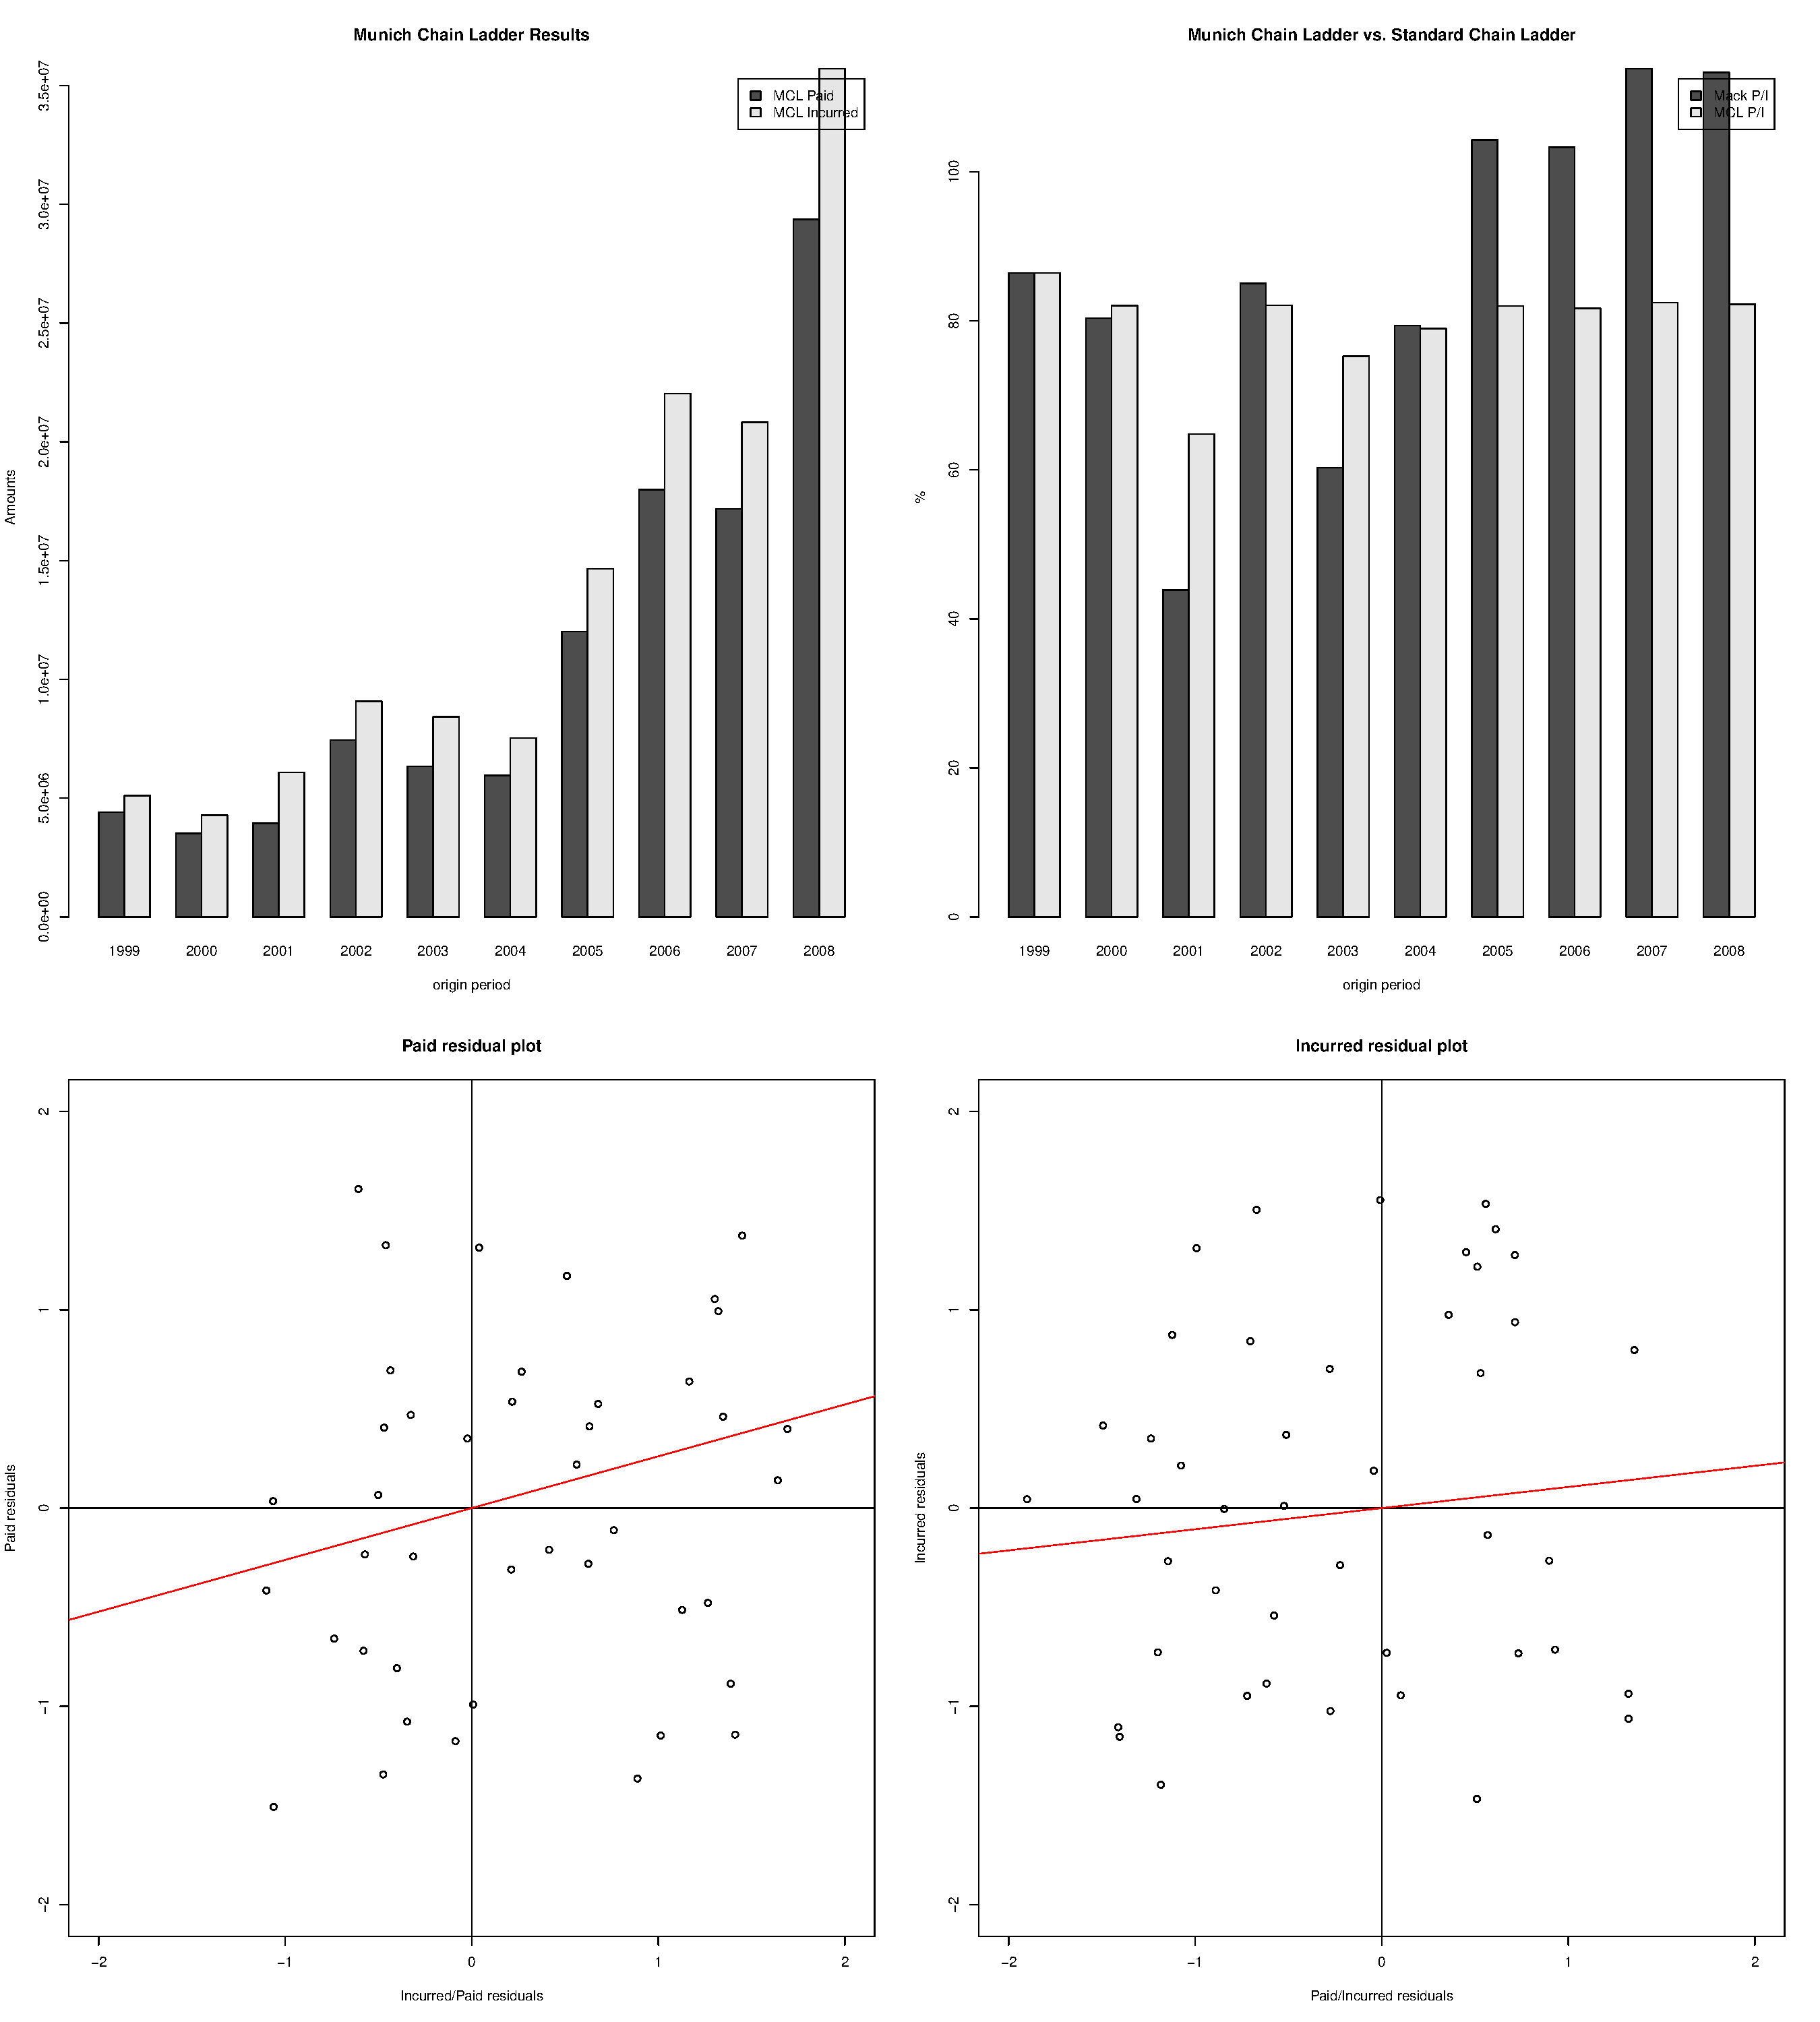
\includegraphics{informe_files/figure-latex/unnamed-chunk-30-1.pdf}
\caption{\label{plotMunich} Gráfico automático para objetos de tipo
Munich Chain-Ladder}
\end{figure}

Al pedir el resumen con la función \texttt{summary} del objeto
\texttt{Munich Chain Ladder} nos devuelve los últimos pagos acumulados y
últimos siniestros incurridos, y el ratio \(P/I\), luego también tiene
las proyecciones de los pagos y de los incurridos mediante el método de
Munich, y el ratio, al pedir que sea por año de origen mediante
\texttt{summary(BayernMunich)\$ByOrigin} esta informacioón nos la
devuelve por año de origen ((tabla \ref{origin Munich})), y se puede
observar como ningún ratio al final de los 10 períodos de desarrollos
supera la unidad.

\begin{table}[ht]
\centering
\caption{Resumen por año de ocurrencia del método Munich Chain-Ladder} 
\label{origin Munich}
\begingroup\fontsize{10pt}{10pt}\selectfont
\begin{tabular}{ccccccc}
  \hline
 & Latest Paid & Latest Incurred & Latest P/I Ratio & Ult. Paid & Ult. Incurred & Ult. P/I Ratio \\ 
  \hline
1999 & 4408012.35 & 5099688.00 & 0.86 & 4408012.35 & 5099688.00 & 0.86 \\ 
  2000 & 3310585.34 & 4221137.00 & 0.78 & 3516429.02 & 4285192.30 & 0.82 \\ 
  2001 & 2183145.17 & 5969088.00 & 0.37 & 3938896.95 & 6078382.19 & 0.65 \\ 
  2002 & 5122735.27 & 8581805.00 & 0.60 & 7450536.68 & 9075686.58 & 0.82 \\ 
  2003 & 2613770.37 & 7276239.00 & 0.36 & 6336075.64 & 8419911.00 & 0.75 \\ 
  2004 & 2244504.33 & 5882585.00 & 0.38 & 5950165.65 & 7535352.06 & 0.79 \\ 
  2005 & 4475502.88 & 9901076.00 & 0.45 & 12013700.59 & 14652550.55 & 0.82 \\ 
  2006 & 5966324.20 & 12548654.00 & 0.48 & 17995072.95 & 22028140.99 & 0.82 \\ 
  2007 & 4760793.00 & 9171465.00 & 0.52 & 17172978.06 & 20825622.64 & 0.82 \\ 
  2008 & 4876379.00 & 10120889.00 & 0.48 & 29364788.76 & 35705671.10 & 0.82 \\ 
   \hline
\end{tabular}
\endgroup
\end{table}

También se puede acceder al resumen pero para el total mediante
\texttt{summary(BayernMunich)\$Totals}, donde se tendrá la suma de las
columnas anteriores, en la primer fila la sumade las diagonales, y su
ratio, y en la segunda lo estimado y su ratio ((tabla \ref{totales}).

\begin{table}[ht]
\centering
\caption{Resumen para el total del método Munich Chain-Ladder} 
\label{totales}
\begin{tabular}{cccc}
  \hline
 & Paid & Incurred & P/I Ratio \\ 
  \hline
Latest: & 39961751.923 & 78772626.000 & 0.507 \\ 
  Ultimate: & 108146656.650 & 133706197.413 & 0.809 \\ 
   \hline
\end{tabular}
\end{table}

Restando la fila `'Ultimate'' menos `'Latest'' de la tabla
\ref{totales}, que refieren a la suma de las estimaciones de los pagos
de todos los años al final de todos los períodos, y la suma de la
diagonal respectivamente se obtiene la reserva de IBNR, que en este caso
se puede obtener para cualquiera de los dos triángulos. Para el
triángulo de siniestros incurridos se tiene que
\(IBNR=133.706.197,413-78.772.626=54.933.951,413\).

Si se estima de esta manera el factor de desarrollo individual para
poder estimar los valores que están enseguida por debajo de la diagonal
invertida, y luego de forma iterativa se completa la matriz, tanto la de
pagos acumulados como la de siniestros incurridos, al final del período,
cuando se evalúen los ratios \((P/I)\) no se obtendrán los valores
mayores a 1 que se obtenían cuando se hacía las dos matrices por
separado.

\section{Bootstrap}\label{bootstrap}

\subsection{Modelado}\label{modelado}

Para la aplicación de bootstrap es necesario primero hacer un modelo
estocástico para la reserva de siniestros incurridos, Kremer (1982)
considera un modelo para el logaritmo de los pagos acumulados, pero
presentaremos el modelo de Poisson sobre-disperso dentro de los modelos
lineales generalizados dado que permite considerar que la varianza no
sea constante para todos los valores predichos. Además, como se verá
luego, es uno de los modelos que acepta la función
\texttt{BootChainLadder}. En este modelo estaremos considerando a la
función logarítmica como función de enlace.

Para los siniestros incurridos del año \(i\) del período de desarrollo
\(j\) (\(I_{i.j}\)) se tendrá:

\[
\mathbb{E}(I_{i,j}) = m_{i,j} \text{   ,    }   \mathbb{V}(I_{i,j})=\phi\mathbb{E}(I_{i,j})=\phi m_{i,j}
\]

\[
log(m_{i,j}) = \eta_{i,j}
\]

\[
\eta_{i,j}= c + \alpha_i + \beta_j  \text{   ,  } \alpha_1=\beta_1=0
\]

En donde \(\alpha_i\) es el parámetro asociado al año de ocurrencia
\(i\) y \(\beta_j\) para el período de desarrollo \(j\), donde se toman
los años y los períodos como `factores', o variables categóricas. Y son
estimados mediante máxima verosimilitud.

Luego, con los valores de \(\alpha_i\) y \(\beta_j\) estimados a partir
del modelo se puede estimar \(\eta_{i,j}\) para los valores de
\(j>c_i\), y se tiene que
\(\mathbb{E}(I_{i,j}) = m_{i,j} = e^{\eta_{i,j}}\) para completar el
triangulo de siniestros incurridos y la reserva de IBNR para cada año.

El otro modelo que acepta la función es el modelo Gamma, que es igual al
modelo Poisson sobre-disperso, solo que la varianza será calcula
\(\mathbb{V}(I_{i,j}) = \phi\cdot \mathbb{E}(I_{i,j})^2=\phi \cdot m_{i,j}^2\).

\subsection{Proceso de Bootstrap}\label{proceso-de-bootstrap}

En 1999 England y Verrall proponen un método de bootstrap a partir de
los modelos antes presentados. Consistene en aplicar el modelo y estimar
los valores de \(\alpha_i\) y \(\beta_j\), luego predecir los valores de
\(I_{i,j}\) del triángulo superior, y calcular los residuos de Pearson
(\(r_p\)).

\[
r_p = \frac{I_{i,j}-\hat{m}_{i,j}}{\sqrt{\hat{m}_{i,j}}}
\]

Luego se aplica Bootstrap sobre los valores de los residuos de Pearson,
y se calculan los valores de siniestros incurridos del triángulo
superior de la forma:

\[
I^*_{i,j} = r^*_p\cdot\sqrt{\hat{m}_{i,j}} + \hat{m}_{i,j}
\] Con la muestra de siniestros incurridos se vuelve a ajustar el modelo
elegido, se calcula el triángulo inferior de la matriz de siniestro y se
calcula la reserva de IBNR para cada año. Este método se repite \(N\)
veces, y el error estandar de las estimaciones será el desvío de los
valores obtenidos en cada muestra de bootstrap.

Por último, el parámetro de escala del desvío \(\phi\) es estimado con
los desvíos de Pearson de la forma:

\[
\phi_P = \frac{\sum r_p^2}{n-p}
\]

Con \(n\) el número de datos en la muestra, que cuando se trabaja con 10
años y 10 períodos son \(55\) datos (el triángulo superior) y \(p\) la
cantidad de parámetros.

\subsection{Aplicación de Bootstrap en
R}\label{aplicaciuxf3n-de-bootstrap-en-r}

Este modelo se aplica con el comando \texttt{BootChainLadder}, que tiene
como argumento los datos (la matriz triangular), la cantidad de muestras
con Bootstrap que se va a obtener (\(R=999\) por defecto), y el modelo
que asumirá, que puede ser el Poisson sobre-disperso o el Gamma
(\texttt{process-distr=c("gamma","od.pois")}) y adicionalmente se le
puede fijar una semilla para replicar los resultados
(\texttt{seed=NULL})

Se puede acceder al resumen de los valores obtenidos tanto para cada año
de ocurrencia (tabla \ref{anual bootstrap}) como para el total, y
obtener los cuantiles para las reservas por IBNR.

\begin{table}[ht]
\centering
\caption{Resumen por año del método Bootstrap Chain-Ladder} 
\label{anual bootstrap}
\begin{tabular}{lcccccc}
  \hline
 & Latest & Mean Ultimate & Mean IBNR & SD IBNR & IBNR 75\% & IBNR 95\% \\ 
  \hline
1999 & 5099688.0 & 5099688.0 & 0.0 & 0.0 & 0.0 & 0.0 \\ 
  2000 & 4221137.0 & 4302459.0 & 81322.0 & 484217.3 & 61837.3 & 691020.2 \\ 
  2001 & 5969088.0 & 6223378.1 & 254290.1 & 856881.0 & 432400.3 & 1350382.5 \\ 
  2002 & 8581805.0 & 9038419.6 & 456614.6 & 1280673.2 & 788443.8 & 1963269.5 \\ 
  2003 & 7276239.0 & 8597099.5 & 1320860.5 & 1456675.5 & 1921733.2 & 4007580.1 \\ 
  2004 & 5882585.0 & 7650991.2 & 1768406.2 & 1646468.4 & 2503223.8 & 4269812.0 \\ 
  2005 & 9901076.0 & 14283851.2 & 4382775.2 & 2864058.8 & 5696647.2 & 8833304.4 \\ 
  2006 & 12548654.0 & 21688448.2 & 9139794.2 & 4480670.1 & 11625445.2 & 16794550.8 \\ 
  2007 & 9171465.0 & 19764014.5 & 10592549.5 & 4768722.6 & 13323177.8 & 18997188.2 \\ 
  2008 & 10120889.0 & 34073750.5 & 23952861.5 & 9370456.1 & 28559335.2 & 40249299.0 \\ 
   \hline
\end{tabular}
\end{table}

\begin{table}[ht]
\centering
\caption{Resumen Para el total del método Bootstrap Chain-Ladder} 
\label{total bootstrap}
\begin{tabular}{lc}
  \hline
 & Totals \\ 
  \hline
Latest: & 78772626.0 \\ 
  Mean Ultimate: & 130722099.8 \\ 
  Mean IBNR: & 51949473.8 \\ 
  SD IBNR: & 18892088.9 \\ 
  Total IBNR 75\%: & 60136149.4 \\ 
  Total IBNR 95\%: & 83350428.8 \\ 
   \hline
\end{tabular}
\end{table}

También se puede obtener el gráfico con la función \texttt{plot} a un
objeto de la clase \texttt{'BootChainLadder'}. En los dos gráficos
superiores de la figura \ref{plotBoot} se obtien el histograma del total
de reservas de IBNR y la función de distribución de las reservas por
IBNR. Mientras que en la parte inferior se obtienen gráficos de
dispersión de los costos últimos simulados para cada año de origen con
la media en rojo y de las simulaciones de los costos acumulados actuales
para cada año, con el valor observado en la diagonal en rojo.

\begin{figure}
\centering
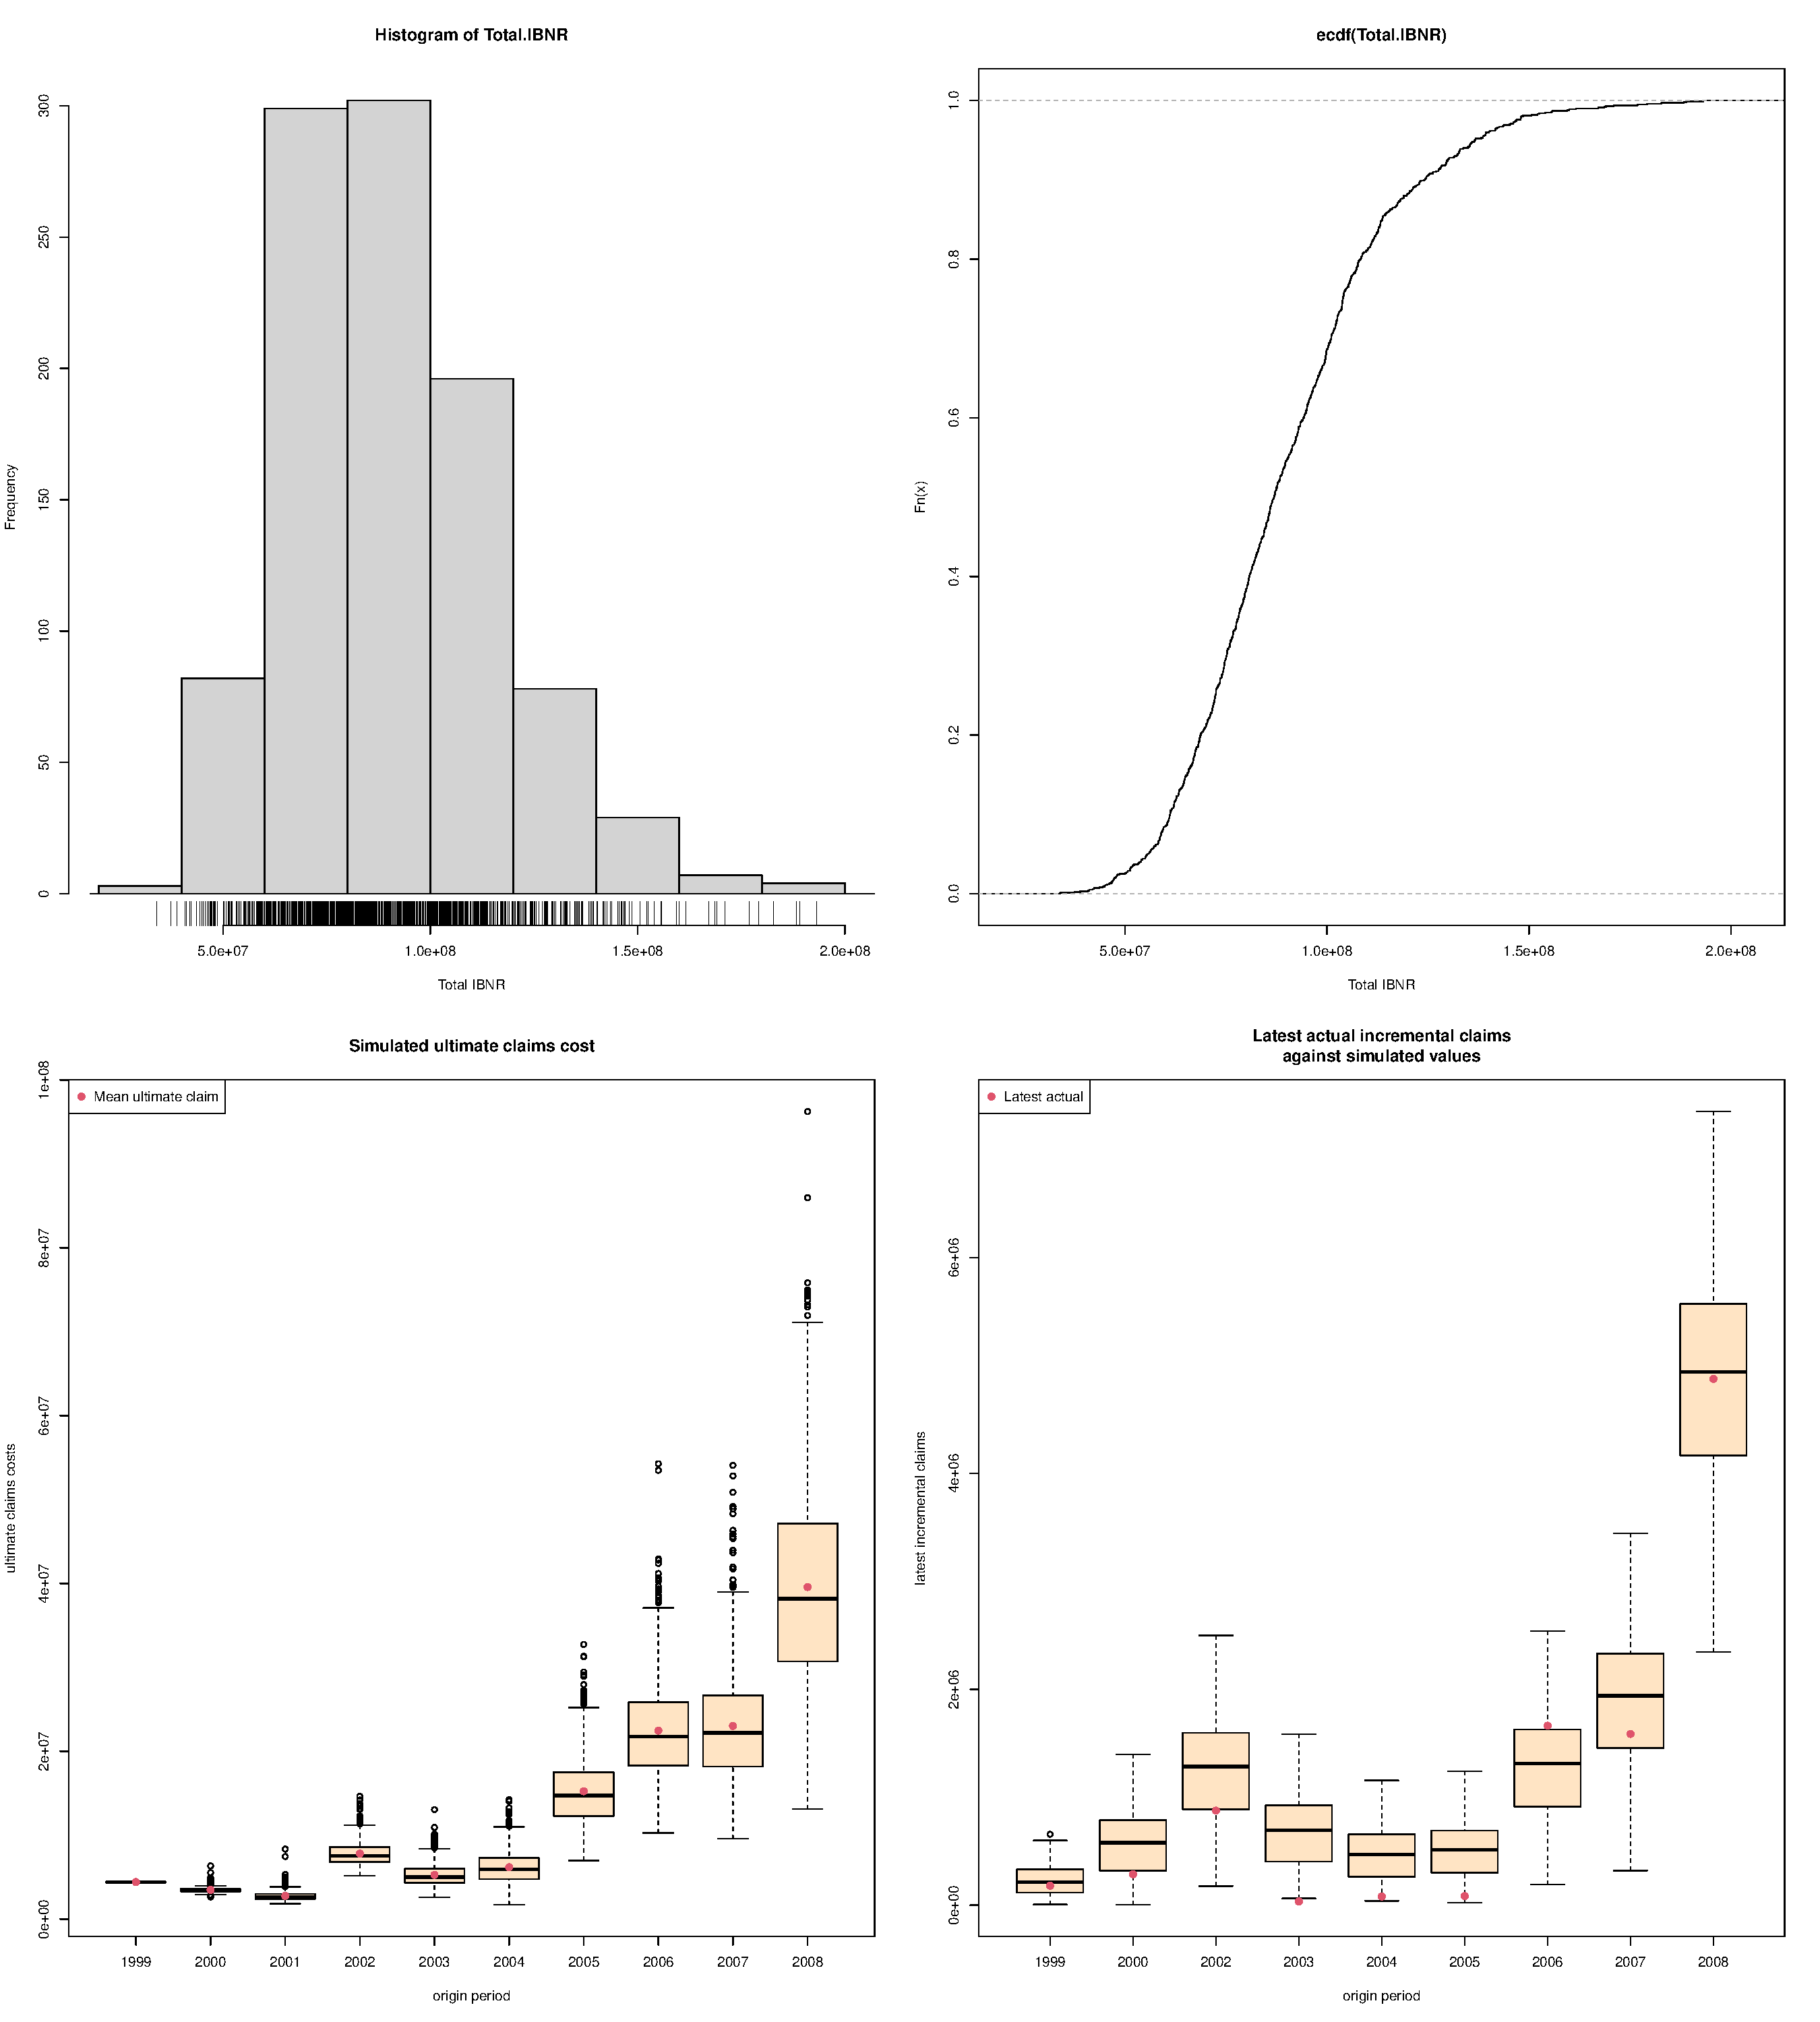
\includegraphics{informe_files/figure-latex/unnamed-chunk-36-1.pdf}
\caption{\label{plotBoot} Gráfico automático para objetos de tipo
Bootstrap Chain-Ladder}
\end{figure}

Además también se pueden obtener los cuantiles de interés para cada año
mediante la función \texttt{quantile} para obtener un intervalo de
confianza al 95\%, ya que la función \texttt{summary} brinda el cuantil
\(0.75\) y el \(0.95\)

\begin{table}[ht]
\centering
\caption{IC al 95 por año del método Bootstrap Chain-Ladder} 
\label{quantile_boot}
\begin{tabular}{lrr}
  \hline
 & IBNR 2.5\% & IBNR 97.5\% \\ 
  \hline
1999 & 0.0 & 0.0 \\ 
  2000 & -696210.4 & 1161331.9 \\ 
  2001 & -905242.5 & 1636852.9 \\ 
  2002 & -1223492.5 & 2680851.3 \\ 
  2003 & -698372.2 & 4870507.5 \\ 
  2004 & -202046.5 & 5012521.1 \\ 
  2005 & 502422.6 & 9766063.0 \\ 
  2006 & 2327520.7 & 19154879.5 \\ 
  2007 & 3388073.5 & 21114968.2 \\ 
  2008 & 7750787.2 & 46071595.3 \\ 
   \hline
\end{tabular}
\end{table}

En la tabla \ref{quantile_boot} se puede observar que para el primer año
de origen se tiene una límite inferior del intervalo negativo, esto se
debe a que la media es 0, y la parte de simulación de los errores se
generan valores negativos, esto se puede arreglar o bien truncando el
intervalo de confianza, o asumiendo que la reserva para el primer año es
0 y no tiene varianza ni desvío.

\section{Comparación de Métodos}\label{comparaciuxf3n-de-muxe9todos}

Como se comentó al principio, durante el documento se pretendía abordar
diferentes métodos para el cálculo de la reserva para siniestros
incurridos pero no reportados, o reserva de IBNR. Para el cálculo de la
reserva de IBNR se contaba con una matriz triangular, que según el caso
podía ser la de siniestros incurridos o la de pagos acumulados, y los
métodos abordados se utilizaban para completar esta matriz, es decir,
para predecir cómo se comportaran los reclamos ocurridos en cada año,
durante el desarrollo de los siguientes años, y así determinar una
reserva para poder cubrir los futuros reclamos.

El primer método que se aplicó fue el `'Chain-Ladder clásico'`, y luego
se tuvo en cuenta una pequeña variación de un'`Chain-Ladder con
regresión'' de los factores de desarrollo a lo largo de los períodos de
desarrollo. Estos dos modelos eran sencillos y fáciles de entender,
además se podían aplicar tanto sobre el triángulo de pagos acumulados
como en el triángulo de siniestros incurridos. Se observó que el modelo
con regresión producía una reserva de IBNR mayor al modelo clásico
debido a que el factor del último período de desarrollo era mayor a uno.
Una de las desventajas de estos modelos es que no se obtenían medidas de
dispersión de las estimaciones y tampoco se podían realizar intervalos
de confianza para las mismas.

El método de `'Mack Chain-Ladder'' utiliza los factores de desarrollo
individuales para cada año de ocurrencia y período de desarrollo, además
brindaba una estimación de los errores estandar de la estimación de la
reserva de IBNR, esta estimación de los errores surge de los errores que
se obtienen para la estimación de los pagos en el último período de
desarrollo, ya que la reserva de IBNR para cada año de ocurrencia era la
resta de estos menos el último pago ocurrido.

Luego, el método de `'Munich Chain-Ladder'' tenía en cuenta la
correlación entre ambos triángulos y se completaba ambos triángulos al
mismo tiempo, por lo que se podía obtener la reserva de IBNR para
cualquiera de los dos, y la varianza se obtenía de una forma parecida al
método de Mack, a través de la varianza de los factores de desarrollo.

Por último, el método de Bootstrap surgía de asumir un modelo para los
pagos acumulados, que podía ser el `'Poisson sobre disperso'' o el
modelo `'Gamma'`, a partir de la predicción de los pagos acumulados se
obtienen a través de bootstrap los residuos de Pearson, se despeja los
valores de pagos acumulados de la fórmula de los residuos, y se
desarrolla el modelo de'`Chainn-Ladder'' con estos valores de pagos
acumulados. Este modelo generaba medidas de la varianza de las
estimaciones, a través de la varianza muestral del Bootstrap.

\subsection{Comparaciones de las Reservas de
IBNR}\label{comparaciones-de-las-reservas-de-ibnr}

En esta sección se pretende comparar los resultados obtenidos de la
aplicación de los distintos métodos, comparar el valor de la reserva de
IBNR entre sí y con respecto al `'Chain-Ladder clásico'', y en los casos
en que haya, comparar las medidas de variación.

Se comparan los siniestros incurridos en la tabla \ref{Comparaciones1}
que cuenta con la última pérdida esperada total para cada método, la
reserva de IBNR, el error y el coeficiente de variación si corresponde,
y el porcentaje en que varía la estimación de la reserva respecto al
Chain-Ladder clásico, en donde se observa que el `'Chain-Ladder con
regresión'' aumenta en un 5,7\% las reservas de IBNR, el `'Mack
Chain-Ladder'' un 0,04\%, el `'Munich Chain-Ladder'' aumenta las
reservas en un 9,7\% y el método de `'Bootstrap'' un 3,7\%.

\begin{table}[ht]
\centering
\caption{Comparación de la Estimación de la última pérdida y de la Reserva de IBNR para los Siniestros Incurridos con distintos métodos, medidos en Millones de pesos} 
\label{Comparaciones1}
\begin{tabular}{lrrrrr}
  \hline
 & Pérdida Esperada (M) & IBNR (M) & Error & CV & VariaciónPorcentual \\ 
  \hline
C-L Clasico & 128.9 & 50.1 &  &  & 0.000 \\ 
  C-L Regresión & 131.7 & 52.9 &  &  & 5.659 \\ 
  Mack C-L & 128.9 & 50.1 & 11156939.5 & 0.22 & 0.041 \\ 
  Munich C-L & 133.7 & 54.9 &  &  & 9.677 \\ 
  Bootstrap & 130.7 & 51.9 & 18892088.9 & 0.36 & 3.719 \\ 
   \hline
\end{tabular}
\end{table}

Se observa que entre los modelos que tenían una medida del desvío el
método de Bootstrap tiene mayor desvío y el coeficiente de variación es
de un 36\%, mientras que el método de Mack tiene un coeficiente de
variación del 22\%, además, en mayor o menor medida todos los métodos
sobre estiman la reserva de IBNR respecto al método clásico, es decir,
dan más seguridad.

\newpage

\section*{Bibliografía}\label{bib}
\addcontentsline{toc}{section}{Bibliografía}

\phantomsection\label{refs}
\begin{CSLReferences}{1}{0}
\bibitem[\citeproctext]{ref-tesis}
Alfaro Fuentes, Daniel de Jesús. 2016. {«Modelos Chain-Ladder clásicos y
bayesianos para el cálculo de reservas auxiliado con R»}. Tesis de
Licenciatura, México: Universidad Nacional Autónoma de México.
\url{https://repositorio.unam.mx/contenidos/291089}.

\bibitem[\citeproctext]{ref-bootstrap}
England, P. D., y Richard Verrall. 2002. {«Stochastic Claims Reserving
in General Insurance»}. \emph{British Actuarial Journal} 8 (agosto).
\url{https://doi.org/10.1017/S1357321700003809}.

\bibitem[\citeproctext]{ref-chain}
Gesmann, Markus, Daniel Murphy, Yanwei (Wayne) Zhang, Alessandro
Carrato, Mario Wuthrich, Fabio Concina, y Eric Dal Moro. 2023.
\emph{ChainLadder: Statistical Methods and Models for Claims Reserving
in General Insurance}.
\url{https://CRAN.R-project.org/package=ChainLadder}.

\bibitem[\citeproctext]{ref-mack}
Mack, Thomas. 1993. {«Distribution-free Calculation of the Standard
Error of Chain Ladder Reserve Estimates»}. \emph{ASTIN Bulletin} 23 (2):
213-25. \url{https://doi.org/10.2143/AST.23.2.2005092}.

\bibitem[\citeproctext]{ref-munich}
Quarg, Gunther, y Thomas Mack. 2004. {«Munich Chain Ladder»}.
\emph{Bl{ä}tter DGVFM} 26: 597-630.
\url{https://doi.org/10.1007/BF02808969}.

\end{CSLReferences}

\end{document}
